%# -*- coding: utf-8-unix -*-
% !TEX program = xelatex
% !TEX root = ../thesis.tex
% !TEX encoding = UTF-8 Unicode

\chapter{面向复杂语义的知识库自动问答研究}
\label{chap:compqa}

本章的研究为基于知识库的自动问答任务。
用户提出的问句可能具有复杂语义,其中包含了未知答案与相关实体的多种关系,
因此复杂问句的回答过程充满了挑战。
我们提出了面向复杂语义的知识库问答模型,
主要特点在于,我们利用神经网络学习复杂语义结构的整体连续特征表示,
从而捕捉不同语义成分之间的信息交互。
%本章提出的模型复杂问题数据集上取得了优秀的结果,
%在多个简单问题数据集上依然保持竞争力。

%Answering complex questions that involve multiple entities and
%multiple relations using a standard knowledge base is an open and 
%challenging task. Most existing KBQA approaches focus on
%simpler questions and do not work very well on complex questions
%because they were not able to simultaneously represent the question
%and the corresponding complex query structure.
%In this work, we encode such complex query structure into a uniform vector 
%representation, and thus successfully capture the interactions between
%individual semantic components within a complex question. This approach
%consistently outperforms existing methods on complex questions while
%staying competitive on simple questions.


%# -*- coding: utf-8-unix -*-
% !TEX program = xelatex
% !TEX root = ../thesis.tex
% !TEX encoding = UTF-8 Unicode

\section{概述}%intro
\label{sec:compqa-intro}


基于知识库的自动问答(KBQA)是自然语言处理中的经典应用场景。
该任务以自然语言问句作为输入,
并根据已有结构化知识库提供的信息,寻找到问句的一个或多个答案。
以Freebase,YAGO,DBPedia为代表的结构化知识库
主要以维基百科为骨架构建而成,它们包含真实世界的广域知识,因此常用于自动问答任务中。

%The knowledge-based question answering (KBQA) is a task which 
%takes a natural language question as input and returns a factual answer 
%using structured knowledge bases
%%organizing open domain facts in the real world,
%such as Freebase~\cite{bollacker2008freebase},
%YAGO~\cite{suchanek2007yago} and DBpedia~\cite{auer2007dbpedia}.
%%organize massive open domain facts in the real world,
%%and make KBQA an open and popular research task,


在自动问答任务中,我们关注的问题称为``{事实类问题}'' ,其特点在于
它们询问的是与句子中实体相关的客观事实,因此答案为知识库中存在的实体、数值或时间。
以一个较简单的问题为例,``What's the capital of the United States?'' ,
为了准确回答这个问题,一个较为直接的方式是,首先识别句子中的相关实体并链接到知识库,
再将该实体与目标答案之间的自然语言关系映射为知识库中的一个谓词(或为词序列),
那么原问题即可转换为具有(实体,谓词,目标答案)三元组形式的查询语句,
例如($united\_states$, $capital$, $?$),通过在知识库上运行查询语句,生成最终的结果。
将已有的\textless 问题,答案 \textgreater 对作为训练数据,
我们可以通过远距离监督(Distant Supervision)的形式学习问句和查询语句之间的映射关系。

%%The questions in KBQA task are factual questions,
%%since the answer of each question is an object entity\footnote{Could be type or literal value}
%%of an existing subject entity in the question.
%One simple example is a question like this: ``What's the capital of the United States?''
%%we need to first recognize the subject named entity in the question,
%%for example, \textit{united\_states} in Freebase,
%%then understand the relation ``capital of'' connecting the subject and object answer,
%%is represented by the predicate \textit{location.location.capital} in FB, for example.
%A common answer to such question is to identify the focus entity
%and the main relation predicate (or a sequence) in the question, and 
%map the question to a triple fact query ($US$, $capital$, $?$) over KB.
%The object answers are returned by executing the query.
%The mapping above is typically learned from question-answer pairs
%through distant supervision.


对于只包含简单语义的问题,我们可以通过上述方法将其转为知识库上的一个基本三元组查询,
但这样的方法并不适用于其它具有更复杂语义的问题。
例如\figref{fig:compqa-intro}所示,为了准确回答问题
``What is the second longest river in United States?'' ,
我们实际上需要对其进行推理,得出以下三条语义线索:
1) 答案实体位于美国内部;
2) 答案实体的类型是河流;
3) 在满足前两个条件的所有实体中,根据长度属性进行降序排列,目标答案排在第二位。
具体分析,第一条语义类似于简单问题,描述相关实体和答案间的关联,
第二条语义则描述了知识库中的特定类型与答案的包含关系,
第三条语义和序数相关,它甚至不能简单地对应到知识库中已有的事实三元组。
由此可见,我们需要挖掘出多条不同的关系,才能准确地定位目标答案。
对于这类无法通过单个三元组查询来精确描述语义的问题,
我们将它称为``{复杂问题}'' ,也是这个章节研究的重点。

\begin{figure}[ht]
	\centering
    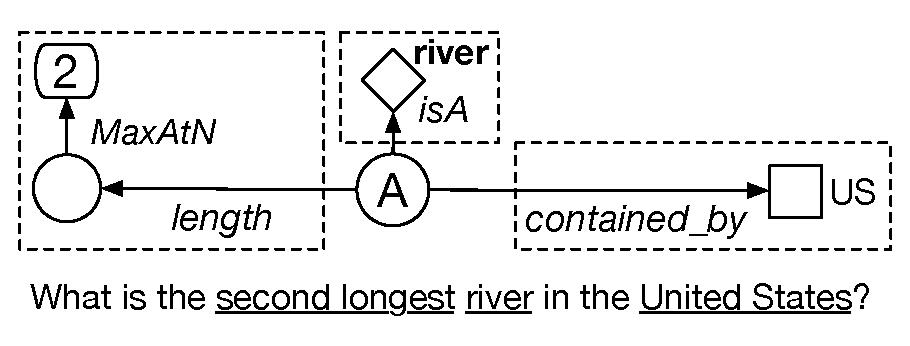
\includegraphics[width=0.7\columnwidth]{figure/compqa/intro.eps}
	%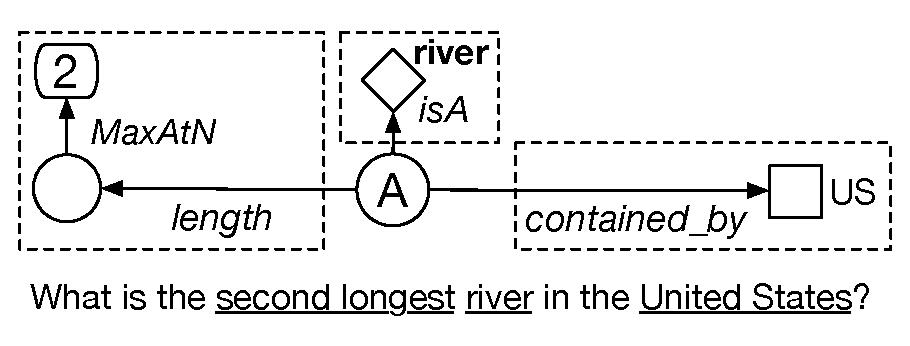
\epsfig{file=figure/compqa/intro.eps, angle=0, width=1.0\columnwidth}
	%\scalebox{0.3}{\includegraphics{overview.eps}}
	\bicaption{一个具有复杂语义的问句示例。}{Running example of complex question.}
	\label{fig:compqa-intro}
\end{figure}

%While the above question can be answered by querying
%a single predicate or predicate sequence in
%the KB, many other more complex questions cannot, e.g. the question
%in \figref{fig:intro}.
%%However, KBQA is not a trivial task,
%%because we are facing questions more complex than the previous case,
%%where the semantics of the question is not expressed by a single triple fact.
%%One question could have several focus entities,
%%like ``Who played Bilbo Baggins in the Hobbits'',
%%where both the character and the film are focus entities.
%%Our running example in \figref{fig:intro} is even more complex,
%To answer the question ``What is the second longest river in United States'',
%we need to infer several semantic clues:
%1) the answer is contained by United States;
%2) the answer is a river;
%3) the answer ranks second by its length in descending order.
%Thus, multiple predicates are required to constrain the answer set,
%and we call such questions ``complex questions'' throughout this paper.
%%According to statistics reported by Bao et al.~\shortcite{bao2016constraint},
%%15\% questions in WebQuestions~\cite{berant2013semantic}, which is a 
%%popular KBQA dataset, are complex.
%%and the ComplexQuestions dataset is designed for measuring the quality
%%of KBQA systems on the complex scenario, where all questions are complex.





回答复杂问题的核心,在于问答系统是否能准确理解问句中多部分语义之间的组合关系,
而不仅仅是通过搜索的方式得到答案。
这条思路对应了解决自动问答的语义解析技术(Semantic Parsing)
\cite{kwiatkowski2013scaling,berant2013semantic}。
对于一个问句,基于语义解析的模型会将其转换成一棵语义解析树,
%CCG:自底向上将句子中的单词组合起来,语法以及语义:基于lambda表达式,
%有些词语充当function,有些则充当argument
%通过预定义的语法,自底向上形成整个树
%将pred和entity都映射到KB,
这样的解析树等价于知识库中的查询图(Query Graph),
与关系理解中的模式图类似,是包含未知实体知识库子结构。
本章中,``{语义解析树}'' , ``{查询结构}'' 和 ``{查询图}'' 表示同一概念。
\figref{fig:compqa-intro}为问题
``What is the second longest river in United States ?'' 的查询图,具有树形结构。
代表未知答案的节点A为解析树的根节点,
三个叶节点$US$,$river$,$2$则由问句的字面描述中抽取出来,
并已链接到知识库中的实体、类型、时间或是数值上。
这些叶节点通过知识库中的谓词(序列)与答案节点连接,
从而对未知答案进行限制,因此本节中也称叶节点为问句的``{相关节点}'' 。
此外,近年来神经网络模型在提高自动问答系统的性能方面显示出了巨大的前景,
在多个不同的自动问答数据集上,通过神经网络改善语义解析的方法成为了目前最先进的技术
\cite{yih2015semantic,bao2016constraint,xu2016question}。
基于以上论述,本章所讨论的工作围绕语义解析技术结合神经网络模型的思路,
并将其扩展至复杂问题场景。

%For answering complex questions, it's more important to understand the compositional
%semantic meanings of the question.
%%rather than directly outputting answer entities.
%As a classic branch of KBQA solutions, semantic parsing (SP) technique
%%Therefore, our research work is based on the semantic parsing (SP) technique
%~\cite{berant2013semantic,yih2015semantic,reddy2016transforming,hu2018answering}
%aims at learning semantic parse trees or equivalent query graphs
%\footnote{The term ``query graph'' is interchangeable
%with ``query structure'' and ``semantic parsing tree'' throughout this paper.}
%for representing semantic structures of the questions.
%For example in \figref{fig:intro}, the query graph forms a tree shape,
%where the focus nodes (\textit{US}, \textit{river}, \textit{2nd})
%are extracted from the mentions of the question,
%and the answer node is connected to these nodes via predicate 
%sequences in the knowledge base.
%%SP-based approaches first generate candidate graphs using
%%bottom up parsing~\cite{berant2013semantic,cai2013large}
%%or staged query generation methods~\cite{yih2015semantic,bao2016constraint}, 
%%then predict the best graph by calcuating the semantic similarity of the question.
%%Final answers are produced by executing the SPARQL query (shown in \figref{fig:intro})
%%translated from the query graph.
%Recently, neural network (NN) models have shown great promise in
%improving the performance of KBQA systems,
%and SP+NN techniques become the state-of-the-art on several KBQA datasets
%~\cite{qu2018question,bao2016constraint}.
%According to the discussion above, 
%our works extends the current research in the SP+NN direction.




%%4. challenge: candgen
%\KZ{Simplify these two challenges significantly.}
%We face two key challenges for answering complex questions.
%First, there is a large searching space to collect candidate query structures.
%For simple questions, the query structure is limited to 
%a single predicate connecting the focus entity and the answer.
%However, as illustrated in \figref{xxx},
%the query structure of a complex question has a tree shape with multiple edges,
%we can generate different candidates exponentially larger than
%the size we generated from simple questions.
%%4-1. other works
%Traditional semantic parsing approaches partially tackle the problem by
%introducing a ``bridge'' operation to merge simple facts into tree structure
%~\cite{berant2013semantic},
%or predefine a number of parsing templates with branches~\cite{bast2015more},
%Candidate structures can be translated from dependency parsing of the question~\cite{reddy2016},
%but it's highly relies on the parsing accuracy,
%and the translation rules need much human prior knowledge.
%There are approaches to circumvent the problem of candidate generation.
%For example, 
%Xu et al.~\shortcite{xu2016question} generated candidates in the form of single fact,
%and leverage unstructured text information to verify whethe a candidate answer
%satisfies other semantic constarints in the question.
%This approach is out of our discussion,
%as it can be regarded as a post-process step in the majority of KBQA frameworks.
%%4-2. yih & bao
%Recently, stagged query structure generation is a technique proved to be effective
%in research works~\cite{yih2015semantic,bao2016constraint}.
%The intuition is to generate query structure in step-by-step extension:
%starting from a focus entity extracted from the question, then explore candidate paths
%to the answer entity, and attach constraint paths in a depth-first search manner.
%
%Staged generation is proved to be effective and used in xxx research works.
%The difference: rules applied for particular constraints.
%
%%yih proposed a staged candidate generation scheme.
%%Based on candidate entities, search from one entity, and add constraints to the tree from other entity.
%%Bao is similar framework, considers entity / type / time / ordinal constraints with few handcrafted rules.
%%stage generation proves to be effective





语义解析模型可以分为两个部分:生成候选查询图,以及预测最佳查询图。
候选查询图的生成可以采用自底向上的方式构建\cite{berant2013semantic,berant2014semantic},
或是分阶段形式,由简到繁逐步生成所有候选\cite{yih2015semantic,bao2016constraint}。
预测最佳查询图,主要是基于计算问题和查询图之间的语义相似度,挑选出最佳查询图。
对于回答简单问题,目前已有的神经网络模型主要遵循 ``{编码-比较}'' 框架,
即首先利用卷积神经网络(CNN)或循环神经网络(RNN),
将原始问题以及候选的谓词序列分别进行编码,形成在同一个向量空间中的两个不同的语义向量,
两者之间的语义相似度则可以定义为向量空间中的距离度量。

当输入的问题具有复杂语义时,候选的查询图无法简化为线性的谓词序列,
如何对复杂的查询图进行编码,成为了语义相似度模型的关键问题。
一个较为直观的做法,是将整个查询图看做由答案节点到不同叶节点的路径集合,
%一个直观的做法,就是将整个查询图拆分为多个部分,%(换个词?)
例如\figref{fig:compqa-intro}中的虚线框将查询图分成三个语义成分,
分别对应指向不同相关实体的谓词序列。
%每个部分仅关心答案节点到一个叶节点的路径,即谓语序列,
%代表一部分的语义
这使得针对简单问题的神经网络模型可以被直接应用,
即分别计算问句与不同语义成分的相似度分值,并将其聚合(平均或相加),
用来代表问句与查询图整体的语义相似度。

这种基于查询图拆分的方式具有其合理性,
每个语义成分仅对应一个相关实体,类似人类对问句推理得到的平行语义线索。
然而,基于此法套用简单问题的神经网络模型,依然存在两个缺陷。
%每条谓语路径可以准确表示问句的部分语义
%有意义 但是优缺点
%这样的做法依然面临两个局限。
第一个缺陷是,将独立的语义成分与问句直接比较会带来风险。
对于简单问题,唯一的谓词路径代表了整个问句的语义,
%在信息量对等的情况下,
问句和查询对应的语义向量越相近,代表它们匹配度也越高。
然而复杂问题的查询图中,每一个独立的路径仅包含问句部分语义,
即便是正确的谓词路径,与问句整体依然存在语义差距。
%准确的来说,这是蕴含问题
若整体相似度由各部分相似度相加产生,则可能导致训练陷入局部极值,
%在没有海量训练数据的情况下,可能导致训练陷入局部极值。
即问句经编码后的语义向量倾向于查询图中的某条特定谓词路径,
而难以和其余正确的语义成分产生匹配。
%相加,有可能倾向于某些特定的路径,而认为其它路径并不正确。
第二个缺陷是,分别计算相似度再简单相加的形式会丢失信息。%(什么样的信息?)
将查询图的多个谓词序列分别进行编码,计算相似度再合并,
这样的做法视作互相独立的多个部分。
因此这样的模型无法理解不同语义成分之间存在的重叠、互补等语义交互。
模型没有学习整个查询图的语义向量,
%模型中没有向量对应整个查询图的语义表示,
因此无法从一个全局的角度描绘复杂查询图所包含的语义组合。

已有的文献\parencite{yih2015semantic,xu2016question}尝试规避上述两个缺陷,
它们的共同点在于从查询结构中仅挑选一条主路径,
与问句计算语义相似度,对于查询结构中的其它限制,
则依赖于人工定义的规则特征,或引入外部非结构化文本进行额外过滤。
问答模型效果得以提升,但并没有直接应对这样的不足。

在本章中,我们着手于利用神经网络模型改善问句与复杂查询图之间语义相似度计算的效果,
并尝试解决之前论述的两个缺陷。
该模型整体基于对问句和谓词序列的编码,将其表示为同一个语义空间下的语义向量。
我们的模型和之前方法主要区别,在于模型对各个语义成分编码后的向量进行结合,
形成对于查询图整体的语义向量表示。
同时,为了弥补问句和语义成分之间的信息不对等,在对问句进行编码的过程中,
我们利用依存语法分析(Dependency Parsing)寻找问句中和特定谓词序列相关的局部信号,
以此作为对问句字面信息的补充,使模型能更好地将问句和不同的语义成分对齐。
%TODO: ensemble和candgen要不在这里也说一下?

%%1. propose
%In order to attack the above limitations, we propose a neural network based 
%%approach to improve relation matching performance of complex question answering.
%approach to improve the performance of semantic similarity measurement
%in complex question answering.
%%\KZ{This is the first time u mention relation matching. Do they understand
%%what it is?}
%%2. basic
%Given candidate query graphs generated from one question,
%our model embeds the question surface and predicate sequences into a uniform 
%vector space.
%%3. combination
%The main difference between our approach and previous methods is that
%we integrate hidden vectors of various semantic components
%and encode their interaction as the hidden semantics of the entire query graph.
%%so that the model  encodes the semantics of whole graph structure.
%%4. dependency
%In addition, to cope with different semantic components of a query graph,
%we leverage dependency parsing information as a complementary of 
%sentential information for question encoding,
%which makes the model better align each component to the question.
%%5. eval
%%the module is able to handle both complex questions and simple questions.
%The contribution of this paper is summarized below.






本章的贡献可以总结为以下四个部分:
\begin{enumerate}
\item{提出了一个轻量化和有效的神经网络模型来解决具有复杂语义的自动问答任务。
据我们所知,这是第一次尝试在模型中对复杂查询图的完整语义进行明确编码;}
\item{通过融入依存语法分析信息来丰富模型中问句的语义表示,
并进行模型分析以验证其有效性;}
\item{通过一种集成的方法,对已有的实体链接工具进行改良,
丰富从问句中获得的候选实体,并进一步提升任务的整体效果;}
\item{在多个自动问答数据集上进行实验,在由复杂问题组成的ComplexQuestions数据集中,
模型的效果超过了已有的方法,在主要有简单问题组成的WebQuestions和SimpleQuestions数据集中,
模型依然具有很强的竞争力。}
\end{enumerate}

% candgen: less rules???? must be kidding me.
% model in general: interactive composing semantic components.
% model in detail: path embedding, rather than predicate word embedding?? (make use of ids and names)
% footnote: http://anonymous.for.double.blind.review

%\begin{itemize}
%\item We propose a light-weighted and effective neural network model to solve complex KBQA task.
%      To the best of our knowledge, this is the first attempt to
%      explicitly encode the complete semantics of a complex 
% 	  query graph (\secref{sec:rm});
%\item We leverage dependency parsing to enrich question representation 
%	  in the NN model, and conduct thorough investigations to 
%	  verify its effectiveness (\secref{sec:qw-repr});
%\item We propose an ensemble method to enrich entity linking from
%      a state-of-the-art linking tool, which further improves the 
%      performance of the overall task (\secref{sec:ensemble});
%
%\item We perform comprehensive experiments on multiple QA datasets,
%      and our proposed method consistently outperforms previous approaches 
%	  on complex questions, and produces competitive results on 
%	  datasets made up of simple questions (\secref{sec:exp}).
%\end{itemize}

%1. compact v.s. separated features (composition is better than isolated calculation) (interaction) (YES INTERATCTION, HOW to state?)
%   a. traditional: yih, xu, jain: ignore or postprocess
%   b. bao: simply weighted sum
%2. "context pattern" or other clues needed to send to the other side of BiCNN (ad-hoc to determine context pattern, not clearly mentioned)
%3. no need pre-train CNN (don't think pre-train is a good choice)

%Main part in the intro:
%  how to tackle the question with multiple constraints.
%  Imitate intro from Yih, Bao, Xu, Jain, Yin(f)...
%
%Interact:
%  semantic interact: (max pooling) simple but effective
%  entity linking: interactive feature (however, not used right now)
%
%RM helped by EL: raw score as evidence
%EL helped by RM: rare (RM is more reliable)

%# -*- coding: utf-8-unix -*-
% !TEX program = xelatex
% !TEX root = ../thesis.tex
% !TEX encoding = UTF-8 Unicode

\section{相关工作}%related
\label{sec:compqa-related}


% \KQ{
% be aware of new papers: \citet{cui2017kbqa},  \citet{hu2018answering},  \citet{abujabal2017automated}. 
% }

% \KQ{
% Part 1: QA system in categories: SP,  IR. 
% For the ``other'' papers like \citet{jain2016question},  \cite{cui2017kbqa}. 
% Brief talk about their main techniques,  in one sentence. 
% Our paper belongs to SP branch. 
% }




基于知识库的自动问答是最近几年的热门研究。
最主要的用于解决自动问答的方法可以分为两类:
基于信息抽取(Information Extraction)和基于语义解析(Semantic Parsing)。

%Knowledge Base Question Answering(KBQA) has been a hot research top in recent years.  Generally speaking,  the most popular methods for KBQA can be mainly divided into two classes: information retrieval and semantic parsing. 




%这里要看一下其他人的related work,FL写的还有些欠缺。
基于信息抽取的问答模型首先通过实体链接寻找句子中的相关实体,
将它们在知识库上邻近的实体抽取出作为候选答案。
对于候选答案的排序,则依赖以候选答案为中心的知识库子图与问句之间的关联特征。
早期的文献\parencite{yao2014information}利用特征工程进行训练,
而后一系列深度学习模型\cite{bordes2014question,dong2015question,hao2017end}
则通过神经网络学习答案在类型、谓词、上下文等多个不同维度与问句的语义关联程度,
并取得了明显的效果提升。
%Information retrieval based system tries to obtain target answer directly from question information and KB knowledge without explicit considering interior query structure.
%There are various methods \cite{yao2014information,bordes2015large,dong2015question,xu2016question} to select candidate answers and to rank results.  
% % treat a KB as a graph connecting different topics and extract the entities in the problem and obtain the knowledge base subgraph centered on those entities.  Each node or edge in the subgraph can be used as a candidate answer,  and the problem vector is extracted by observing the problem according to certain rules or templates.  The final answer can be selected from candidate answers with the help of problem vector.  IR method has the advantage of easy training and fast speed.  
% % However,  due to the lack of semantic encoding,  features in IR methods are hard to interpret and solve complex questions. 
基于语义解析的系统则会先生成带有复杂结构的候选查询图,
将查询图翻译为能在运行在知识库上的结构化查询语句,得到最终的答案。
%直接转换为查询图(DCS,以及之后的办法)
%早期:CCG作为中间过渡
早期的语义解析系统\cite{kwiatkowski2013scaling,cai2013large}根据PCCG文法
生成和具体知识库无关的中间表达形式,通常以$\lambda$算子的形式呈现,
再将$\lambda$算子中的谓词和常量,映射到知识库中的具体谓词和实体。
Liang提出的$\lambda$-DCS\cite{liang2013lambda}是对PCCG的简化,
语义解析树依然为自底向上的方式,但$\lambda$表达式由简单的相交、合并等规则生成,
大大降低了解析树生成的复杂程度。
最近的研究中,分阶段候选差选图的生成\cite{yih2015semantic,bao2016constraint}已证明了其有效性,
它利用深度搜索,通过由简到繁逐步扩展查询图,
不需要定义操作,也摆脱了自底向上生成过程中,组合顺序与单词顺序相关的限制。

%TODO:还是需要再调整,这个语句粗略了。
%TODO:聊一下cui2017和hu2018,还是要靠自己聊。

%Semantic parsing based approach focuses on constructing a semantic parsing tree or equivalent query structure that represents the semantic meaning of the question.  In terms of logical representation of natural language questions,  many methods have been tried,  such as query graph~\cite{yih2014semantic,yih2015semantic} or RDF query language~\cite{unger2012template,cui2017kbqa,hu2018answering}.  
%% For example,  (Yih et al. ,  2014~\cite{yih2014semantic}; Golub et al. ,  2016~\cite{golub2016character}; Yu et al. ,  2017~\cite{yu2017improved}) are based on Freebase. 

% \KQ{Cannot quite get the point of this paragraph. }
% One drawback of traditional semantic parsing method to sovle KBQA problem is that it needs to generate queries based on large amount of entities and predicates in the KB,  a large proportion of which are unseen during the training process.  Therefore,  some research has focused on solving this issue.  One solution is embedding based method,  which represents entities and relations in vector space and predict soundness of candidate triplets from these latent vectors,  such as  
% TransE(Bordes et al. ,  2013)~\cite{bordes2013translating},  TransH~\cite{wang2014knowledge},  TransR~\cite{lin2015learning} and other enhanced but similar models.  The general idea behind these models is training embedding vectors of entities and relations by the formula $h+r\simeq t$.  Besides,  recent work has also focus on character-level model to enhance the performance,  such as (Golub et al. ,  2016).  Golub uses character-level modeling to handle traditional out-of-vocabulary(OOV) problem.  Furthermore,  there are some research on combination of knowledge base and open vocabulary to improve semantic parsing performance.  For example,  (Gardner et al. ,  2017)~\cite{gardner2017open} try to leverage the information contained in both a formal KB and a large corpus to avoid the limit of the schema of the underlying KB.  \citet{qu2018question} goes even further.  It use RNN to capture semantic-level information in question and use an attention mechanism to keep track of the entities and relations in the same time.  However,  most of these approaches can only deal with single-relation questions,  having no ability to deal with ordinal questions and multi-relation questions,  such as ComplexQuestions.  

% \KQ{
% Part 2: NN techniques in QA system. 
% Could briefly talk about KB embedding based approaches,  check \citet{hao2017end} for more information. 
% Many works used NN techniques,  including Xu,  Yih,  Bao,  and lots of SimpQ papers. 
% Try talk about multiple papers in one or two sentences. 
% Bao is most similar to us,  could talk more,  but not so much. 
% Our main difference: encode multiple relations (paths) into a uniform query structure representation (semantic composition).  
% }

随着深度学习的发展,神经网络模型被广泛使用于知识库上的自动问答任务,并且展示出了优秀的结果。
这些方式的基本思路是利用神经网络的对特征表示的学习能力,将问句转换为连续空间上的
向量表示,同时再将查询结构(或答案实体)映射到同一语义空间,
并定义问句和答案的语义相似度,根据\textless 问题,答案\textgreater 对进行学习,
预测正确的查询。
处理简单语义的神经网络问答模型具有较多的变种,
例如
文献\parencite{yin2016simple,golub2016character}使用了字符级别的循环神经网络以及注意力机制,
对谓词序列和相关实体均进行相似度计算,对于未在训练数据中观察到的单词,模型依然具有鲁棒性;
Bordes等人\cite{bordes2014open}利用知识库向量学习,
关注候选答案的在知识库中的类型、相连谓词、相邻实体等信息,
学习它们在知识库上的向量表示,并以此对候选答案进行编码;
Yu等人\cite{yu2017improved}引入了多层循环神经网络,并通过残差连接的方式,
同时捕捉问句在词级别和整体级别与特定谓词序列的语义匹配;
Qu等人\cite{qu2018question}提出了AR-SMCNN模型,
除了利用循环神经网络捕捉问句和谓词序列在语义上的相关性,
还利用了类似与卷积神经网络处理二维图像的方式,
在词级别相似度矩阵中寻找纹理,学习问句和谓词序列的另一种相似度量。

%Recently, as the development of deep learning,
%NN-based approaches have been combined into the KBQA task \cite{bordes2014open}, showing promising result.
%These approaches tries to use neural network models to encode both questions and answers (or query structures) into the vector space.
%Subsequently, similarity functions are used to select the most appropriate query structure to generate the final answer.
%%In NN-based approaches,  different methods for the crucial step, learning representations of questions and answers(or query structures), have been tried,  especially for simple questions.
%For example,
%\citet{bordes2014open}  focuses on embedding the subgraph of the candidate answer;
%\citet{yin2016simple}  uses character-level CNN and word-level CNN to match different information;
%\citet{yu2017improved} introduces the method of hierarchical residual RNN to compare questions and relation names; 
%\citet{qu2018question} proposes the AR-SMCNN model, which uses RNN to capture semantic-level correlation and employs CNN to extract literal-level words interaction. 
% %  \citet{dong2015question}) takes the context and the type of the answer into account

%讲道理,Cui和Hu的论文也要在这里讨论一下
对于利用神经网络回答复杂语义的问题,已有的工作进行了不少尝试,
但并没有尝试学习查询图整体的语义表示。
例如文献\parencite{yih2015semantic,xu2016question}
侧重于用神经网络计算问句和查询图中主路径的匹配关系,相当于退化至简单语义场景。
对于查询图中,除去主路径的其余语义成分,
Yih等人\cite{yih2015semantic}利用人工定义特征捕捉少数特殊语义,
但基于特征工程的方法不具有较好的扩展性;
Xu等人\cite{xu2016question}则挖掘非结构化文本中的上下文信息,
对满足主路径的候选答案进行过滤,这种方式被视为模型计算之后的处理,而并没有从本质上解决问题。
Bao等人\cite{bao2016constraint}利用每个相关实体在问句中的上下文窗口表示局部语义,
并和查询图中的对应的谓词路径进行相似度匹配计算,但谓词路径之间仍缺少关联。


%Belonging to NN-based semantic parsing category, 
%our approach employs a novel encoding structure method to solve complex questions.
%Previous works such as \citet{yih2015semantic} and \citet{bao2016constraint}
%require a recognition of a main relation and regard other constraints as variables added to this main relation.
%Unlike their approaches, our method encodes multiple relations (paths) into a uniform query structure representation (semantic composition),  which allows more flexible query structures. 
%% To handle multi-relation questions,  recent research has focused on NN-based semantic parsing method.  This approach tries to use RNN or CNN network models to encode both questions and query structures into vector space.  Subsequently,  similarity functions,  such as cosine similarity or dot product,  can be used to select the most appropriate query structure to generate final answer.  For example,  the MulCG (Bao et al. ,  2016)~\cite{bao2016constraint} requires a recognition of a core chain and regards other constraints as variables added to this main relation.  After,  the MulCG uses Siamese CNN to calculate the similarity of question embedding and schema embedding to rank candidate query structures.  The latent problem is (1) six patterns are not adequate to support all kinds of multi-relational questions,  (2) answering all sub-questions separately can be redundant and (3) they can't solve ordinal questions until the final answer refinement step.  However,  this final step adds an additional resource wikipedia to select one answer from possible candidate answers,  which is not only slow but easy to mismatch.  Compared to the MCCNN,  our model avoids redundant work to answer sub-questions successively by fully representing the multi-relational question in a uniform way.  Besides,  our schema treats the ordinal constraints and other constraints equally thus don't need extra work like the refinement step. 

此外,依存语法分析可以描述一个句子中,词汇间的远距离依赖关系,
考虑到它与查询图的结构较为相似,
因此候选查询结构的生成可以基于依存分析树进行转换,
语义匹配过程也更多利用了结构上的相似关系,
例如文献\parencite{reddy2016transforming,hu2018answering}。
我们的模型同样使用了依存语法分析,但将其视为语义特征的信息来源,
而并非直接决定候选查询图的形状,因此我们可以生成更灵活的查询图。
%(这话可以反着说,别人怎么怎么不好)(或者说,如何优雅的xxx,成为了。。。的问题)

%
% \KQ{
% Part 3: Other related papers from solving complex questions,  mainly non-NN based. 
% Checkout these papers: \citet{reddy2016transforming},  \citet{hu2018answering},  \citet{abujabal2017automated}. 
% All of them used dependency information,  which is similar with ous. 
% our difference: dependency as feature,  not decide the shape of query structures, 
% which allows more flexible query structures. 
% }




%这一段简直了,写的啥玩意儿。。。

%There are also some works can't be simply classified in to IR based methods or SP based methods.   \citet{jain2016question}  introduces Factual Memory Network,  which tries to encode KB and questions in same word vector space,  extract a subset of initial candidate facts,  then try to employ multi-hop reasoning and refinement to find a path to answer entity.   \citet{reddy2016transforming},  \citet{abujabal2017automated}, and \citet{cui2017kbqa} try to interpret question intention by templates,  which learned from KB or QA corpora.   \citet{talmor2018web}  attempts to answering complex questions by decomposing them into a sequence of simple questions. 




% However,  due to the limit of data and the complexity of knowledge graph,  the results of these methods are not very competitive.  
%  

 % However,  it seems inflexible in the MulCG that this model manually classifies constraints into 6 types and needs to determine a main path. 

 % requires a recognition of a core chain (Yih et al. ,  2015~\cite{yih2015semantic}; Bao et al. ,  2016~\cite{bao2016constraint}; Yu et al. ,  2017) and  they regard other constraints as variables added to this main relation.  The MulCG (Bao et al. ,  2016) handles multiple constraints systematically and expands non-entity constraints which develops the staged graph (Yih et al. ,  2015).  However,  they all treats constraint a variable added to a node of main relation,  while our model doesn't have to detect the main relation and treats constraints and relations parallel.  Moreover,  our model is word-based,  in other words,  we don't need KB information to generate our schema.  Our model represents every path a word sequence ended with the final answer entity and merges them together to form an overall schema.  The word sequence path only takes word features into account thus concise and uniform thus prevent an overfit problem. 

% In terms of schema generation,  the MulCG (Bao et al. ,  2016) is not flexible enough by mapping explicitly the exact word proof to detect and match constraints,  while our model applies the attention mechanism which can collect other textual evidences to help detecting constraints. 

% For the model and the ranking step,  the MulCG (Bao et al. ,  2016) embedss question and schema together in feature-based then uses learning to rank,  which requires feature engineering thus not flexible.  And our model embeds respectively question(word-based RNN) and schema then trains with neural networks to get a score. 

% The MCCNN (Dong et al. ,  2015~\cite{dong2015question};Xu et al. ,  2016~\cite{xu2016question}) proposed a dependency tree based method to handle multi-relational questions.  They decompose the original question into simple sub-questions using six dependency patterns,  and the intersection of answer sets of all the sub-questions will be selected as the final answer.   

%Attention
% The attention mechanism~\cite{vaswani2017attention} is widely used for NLP tasks in recent days. (Yin et al. ,  2017~\cite{yin2017type}).  

% % IARNN (Wang et al. ,  2016)~\cite{wang2016inner} is an inner attention RNN that the attention was imposed directly to the input therefore can avoid biased attention problem caused by outer attention RNN.  Nevertheless,  it is unidirectional  and it doesn't consider the mutual influnce of the question and the answer. 
 
% % The ABCNN model proposed by (Yin et al. ,  2015)~\cite{yin2015abcnn} integrates attention into CNNs in order to solve sentence pair modeling problem.  This ABCNN model sets up mutual influence between the sentence pairs into CNNs,  therefore the output embedding of each sentence contains the information of its counterpart.  This ABCNN model gives an intuition of cross attention which takes mutual influence into account. 
 
% Hao~\cite{hao2017end} proposes another cross attention model focus on KBQA task.  This cross-attention mechanism consists of two parts: one answer-towards-question attention part and one question-towards-answer attention part.  It focuses on different answer aspects of each question word and calculates the similarity score of the question and the four different candidate answer aspects.  The final score will be composed of the weighted sum of these four similarity score.  This model well develops the attention mechanism,  however,  the mutual interaction is still not fully established.  The reason lies below:  The four similarity vectors between question and answer aspect are independent to each other thus the mutual influence can't be fully expressed.  
 
% Our cross attention mechanism aims to represent both the question and the schema in a dynamic way.  We take each question word's embedding and each skeleton embedding as input and we import an attention matrix.  For the attention matrix,  each item $e_{ij}$ of this matrix denotes the weight of the \emph{i}-th skeleton and the \emph{j}-th question word.  Thus the \emph{i}-th row represents the contribution of each question word to the \emph{i}-th skeleton,  while the \emph{j}-th row represents the contribution of the \emph{j}-th question word to each skeleton.  This cross-attention mechanism fully takes the mutual influence of the question and the schema into account,  thus generates a more precise and meaningful representation of the schema.  

% In conclusion,  our model has a uniform framework,  and it is concise and flexible, also puissant to answer ordinal questions. 





%加一段我们与它们的区别,就像PL那样
%Unlike their approaches, our method encodes multiple relations (paths) into a uniform query structure representation (semantic composition),  which allows more flexible query structures. 


%============================================================%

\section{我们的方法}%xxxx模型  %approach
\label{sec:compqa-approach}

本节将具体阐述复杂语义下的自动问答模型。
主要包括四个部分:
\begin{enumerate*}
\item{基于分阶段的方式生成所有候选查询图;}
\item{通过神经网络定义问句和查询图整体之间的语义相似度;}
\item{基于集成的方式对已有的实体链接结果进行扩充;}
\item{具体的训练以及测试流程。}%就是paper里面没有提及的细节(分拆F1 list)
\end{enumerate*}

%In this section, we present our approach for solving complex KBQA.
%First, we generate candidate query graphs by staged generation method (\secref{sec:candgen}).
%Second, we measure the semantic similarities between the question and each query graph using deep neural networks (\secref{sec:rm}).
%Then we introduce an ensemble approach for entity linking enrichment (\secref{sec:ensemble}),
%Finally, we discuss the prediction and parameter learning step of this task (\secref{sec:train}).

%# -*- coding: utf-8-unix -*-
% !TEX program = xelatex
% !TEX root = ../thesis.tex
% !TEX encoding = UTF-8 Unicode


\subsection{分阶段查询图生成}
\label{sec:compqa-candgen}
%TODO:先翻译,之后可以讲细一些,包括schema的定义,包括伪代码

本节中主要阐述分阶段候选查询图的生成过程。
与已有的工作比较,例如文献\parencite{bao2016constraint},
我们对候选生成的策略进行了优化,主要利用了查询图中对答案类型的隐含限制,
以及知识库中用来维护和时间段事实相关的特殊设计。
%The constraints that we can handle
本文中,我们主要考虑四种不同的语义限制,
分别是实体、类型、时间、顺序限制。
例如在问句中,实体限制描述了答案与某已知实体的联系,
顺序限制描述了答案按某种方式排序所具有的序号。
%我们更好地利用了知识库的类型信息,帮助过滤偏离查询图语义的类型限制,同时利用知识库对时间段事实的描述方式,
%(结果中配套显示我们的candgen结果高了多少,顺便还可以调整K画一些东西)
以\figref{fig:compqa-candgen}为例,
我们通过问句 ``who is the youngest president of the united states after 2002?''
阐述候选图的具体生成过程,该问句同时包含了上述四种语义限制。
为了方便描述,本节假设Freebase为问答系统所使用的知识库。

%  %it's a common practice to generate all possible query graphs through
%  %multiple stages~\cite{yih2015semantic,bao2016constraint}.
%  %Intuitively, the generation process begins from
%  %extracting candidate focus nodes in the question using linking tools.
%  %Then we connect the answer node to the corresponding focus entity
%  %using predicate sequences in KB.
%  %We call it ``main path'' and it is the basis of more complex structures.
%  %Further, we attempt to attach more constraints to the main path,
%  %%which are represented predicate sequences connect the remaining focus nodes to the main path,
%  %leading to complex query graphs in a tree shape.
%  %%The main intuition is to first find focus entities as the starting point of all candidate structures,
%  %%then extract main paths, and finally enrich the main path by adding different kinds of constraints.
%  We illustrate our staged candidate generation method in this section.
%  Compared to previous mathods, such as \citet{bao2016constraint}, we employ a more effective candidate
%  generation strategy, which takes advantage of implicit type information in query graphs
%  and time interval information in the KB.
%  In our work, we take 4 kinds of semantic constraints into account:
%  \textbf{entity}, \textbf{type}, \textbf{time} and \textbf{ordinal} constraints.
%  \figref{fig:candgen} shows a concrete example of our candidate generation.
%  For simplicity of discussion, we assume Freebase as the KB in this section.
%  %by performing SPARQL querys : generate main path first, and enrich add different kinds of constaints.


\begin{figure*}
	\centering
    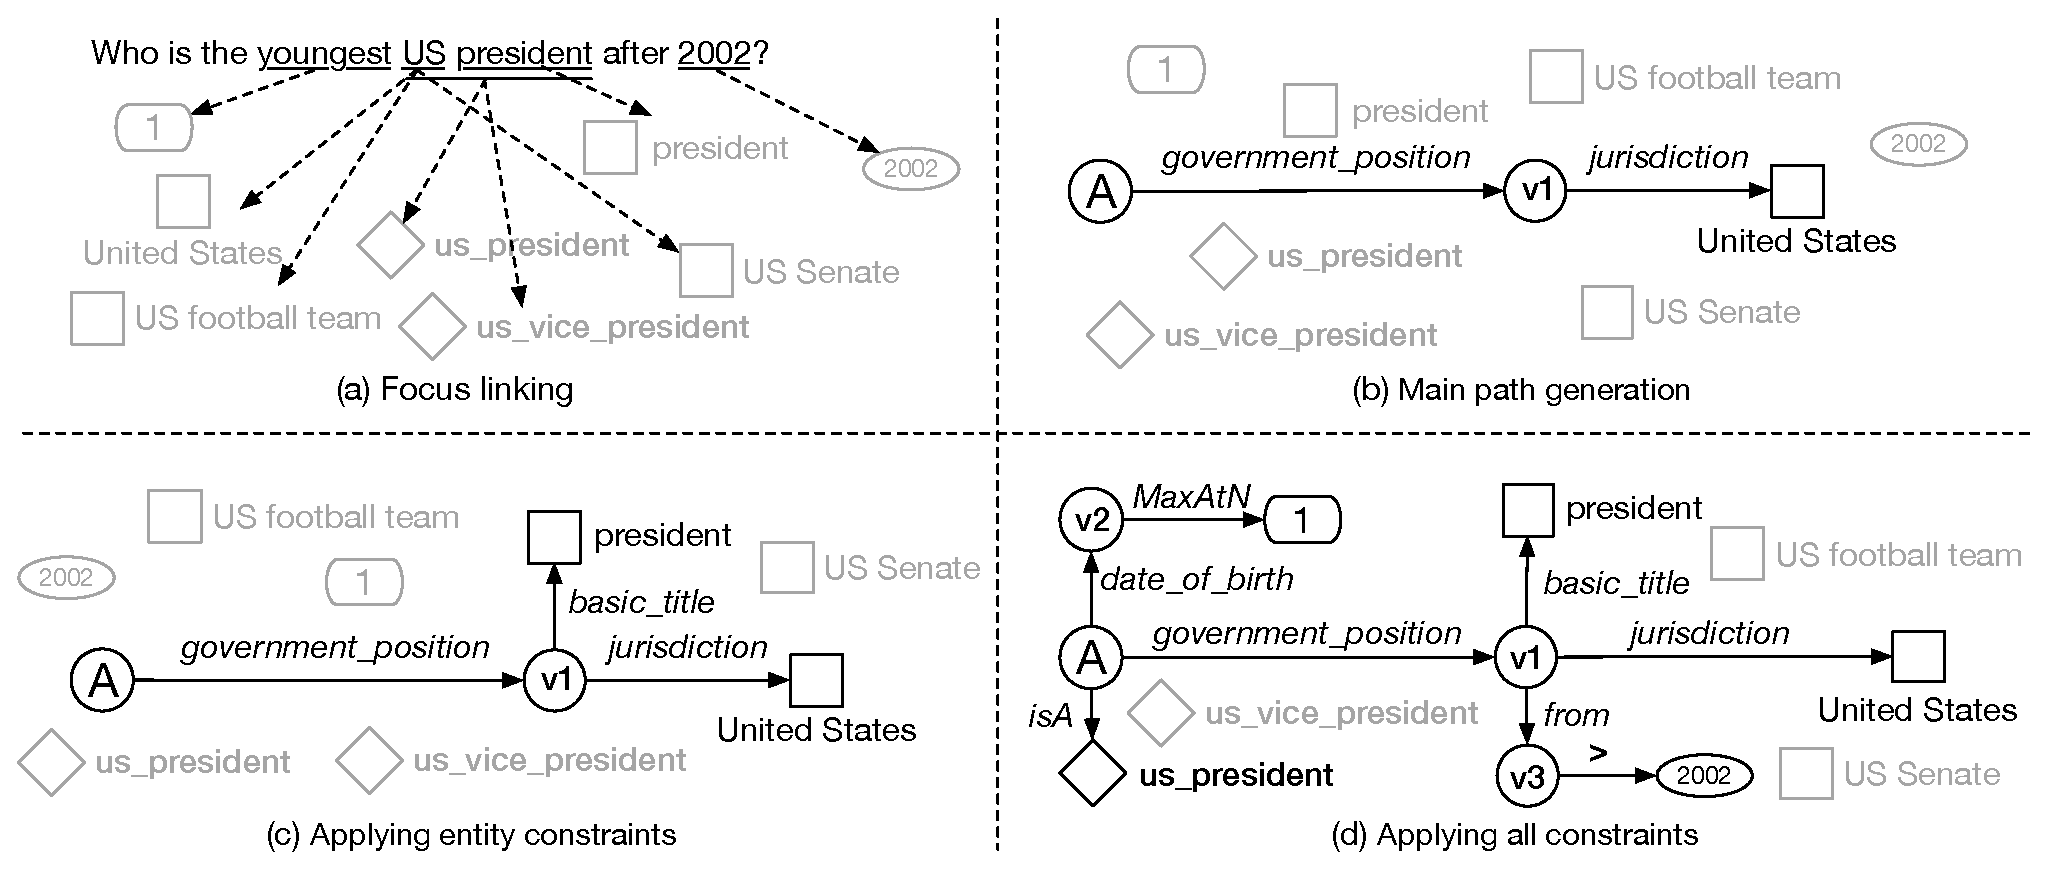
\includegraphics[width=1\columnwidth]{figure/compqa/cangen.eps}
	\bicaption{分阶段候选图生成的具体例子。}{Running example of candidate generation.}
	\label{fig:compqa-candgen}
\end{figure*}


\textbf{阶段一:相关节点链接。}%(最好别叫相关实体,要区分focus和entity)
该步骤寻找问句中代表相关实体、类型、时间、顺序的词汇或短语,并链接到知识库上。
相关节点作为候选查询图的叶节点,是不同类别语义限制的起点。
\figref{fig:compqa-candgen}(a)列出了可能的\textless 短语,叶节点 \textgreater 对,
同一个短语可以对应到多个候选叶节点。
不同语义限制类别(实体、类型、时间、顺序)的叶节点有着各自的链接方式。
对于实体链接,我们使用了已有的链接工具S-MART\cite{yang2015s},
在多个已有的自动问答研究均被使用。
S-MART对所有可能的\textless 短语,实体 \textgreater 进行打分,并保留了至多前十组结果。
对于类型链接,考虑到知识库中不同的类型数量有限,
我们枚举问句中所有长度不超过3的短语,
并根据预训练的词向量,计算不同短语和类型之间的余弦相似度,
同样保留至多前十组结果。
对于时间链接,我们通过正则表达式识别句中出现的所有年份。
对于顺序链接,我们利用预先定义的形容词最高级词汇列表
(例如largest,highest,latest等描述客观事实的最高级词汇),
并在问句中匹配最高级词汇,或 ``{序数词+最高级}'' 的词组,如 ``second longest'' 。
对应的叶节点表示顺序值,若匹配到序数词,则顺序值为序数词对应的数字,否则为1。
如\figref{fig:compqa-candgen}(a)所示,\textless ``youngest'', 1 \textgreater
为生成的唯一顺序链接。

%  \textbf{Step 1: Focus linking.}
%  %This step takes the question as input, and returns candidate (mention, focus) pairs,
%  %where focus node 
%  %for example, (``United State'', \textit{united\_states})
%  We extract possible (mention, focus node) pairs from the question.
%  %We extract possible focus mentions (words or phrases in the question)
%  %and link them to nodes in KB or literal values.
%  Focus nodes are the starting points of various semantic constraints,
%  refer to \figref{fig:candgen}(a).
%  %for example in \figref{fig:candgen}(a),
%  %we link ``US'' to the entity \textit{united\_states},
%  %or ``US president'' to the type \textit{us\_president}.
%  %Different linking methods are used for different categories of focus nodes.
%  %For entity linking, we adopt a state-of-the-art linking tool, S-MART~\cite{yang2015s},
%  %which is widely used in previous KBQA researches.
%  %it scores candidate (mention, entity) pairs based on statistical features from Wikipedia,
%  %such as the lexical similarity, link probability and entity popularity.
%  %The output is a list of (mention, entity) with linking scores,
%  %and one mention can link to multiple entities.
%  For entity linking, we generate (mention, entity) pairs
%  using the state-of-the-art entity linking tool S-MART~\cite{yang2015s}.
%  %trained on Twitter corpus.
%  %Following the S-MART results provided by Yih et al.~\shortcite{yih2015},
%  %up to 10 top-ranked (mention, entity) pairs will be returned.
%  %One mention could lead to several entities.
%  %For example, the mention ``Star Trek'' links to several possible films in the result.
%  For type linking,
%  %due to the limited number of types in Freebase,
%  %we propose a simple but effective method for extracting (mention, type) pairs.
%  %we perform an embedding based brute force search.
%  we brutally combine each type with all uni-, bi- and tri-gram mentions in the question,
%  and pick top-10 (mention, type) pairs with the highest
%  word embedding similarities of each pair.
%  %we enumerate all uni-, bi- and tri-gram mentions of the question,
%  %and calculate the cosine similarities of averaging word embeddings
%  %between the mention and all the type names.
%  %Top-10 scoring (mention, type) pairs are kept as type linking results.
%  %and pair them with all the types in Freebase.
%  %For each (mention, type) pair, we calculate the cosine similarity
%  %of averaging word embedding vectors between them,
%  %and keep top-10 scoring pairs as type linking results.
%  For time linking, we extract time mentions by simply matching year regex.
%  For ordinal linking, we leverage a predefined superlative word list
%  \footnote{A list containing ~20 superlative words, such as largest, highest, latest.}
%  and recognize mentions by matching superlative words,
%  or the ``ordinal number + superlative'' pattern.
%  %``superlative'', ``ordinal number + superlative'' or ``superlative + adjective''.
%  The ordinal node is an integer representing the ordinal number in the mention.
%  %For example, we retrieve (``youngest'', 1) in \figref{fig:candgen}(a).



\textbf{阶段二:生成主路径。}
主路径是一个查询图的基础,代表着问句最主要的语义。
考虑到几乎所有的事实类问题都和问句中至少一个实体相关,
因此它被定义为从答案出发,通过谓词序列连接至某个实体节点的路径,
等同于一个简单问题的查询图。
我们枚举所有被链接的实体,以及它们在知识库中相连的合法谓词序列,
即可生成一系列候选主路径。
谓词序列的长度为1或2,后者实质是描述了多元关系中某两个实体的关联。
%通过知识库中的中间节点\footnote{Freebase中用于维护多元关系的辅助节点。}过渡。
\figref{fig:compqa-candgen}(b)显示出了某一个主路径,
其中答案节点$A$以及中间节点$v1$都是变量节点。%(是不是要多说几句?)
对于后续更复杂的语义限制,在图中均表示为由主路径上某变量节点出发,
指向特定的叶节点的谓词序列。

%  \textbf{Step 2: Main path generation.}
%  %We first build coarse query graphs by using focus entities only, since almost all factoid questions
%  %are related to at least one entity (except corner cases like ``Who's the fastest man in the world?'').
%  %The output of this step is refer to \figref{fig:candgen},
%  %where: one ore more entities are linked to the answer entity by FB predicates in a tree shape.
%  %For constructure different tree shapes,
%  We build different main paths by connecting the answer node to different focus entities
%  using 1-hop or 2-hop-with-mediator
%  %we first pick one focus entity and link the answer node to it by 1-hop or 2-hop-with-mediator
%  \footnote{Mediator is a kind of a auxiliary node in Freebase, used to maintain N-ary facts.}
%  predicate sequence.
%  \figref{fig:candgen}(b) shows one of the main paths.
%  Further constraints are attached by
%  %In the perspective of query graphs, a constraint is represented as a predicate sequence
%  connecting an anchor node $x$ to an unused focus node through predicate sequences,
%  where the anchor node $x$ is a non-focus node in the main path
%  ($A$ or $v_1$ in the example).
%  




\textbf{阶段三:添加额外实体语义限制。}
这个步骤的目的是在主路径之上扩充与实体相关的语义限制。
%所有出现的实体都可能会被用上
%深度搜索:
%枚举位置,连接位置,谓词,若有某种实例化方式,
%使得替代之后,均对应已存在的事实,则添加的限制有意义,引入新的实体,递归操作
受到\secref{sec:schema-candgen}中复杂模式图生成的启发,
我们同样采用深度优先搜索的方式,由简到繁进行查询图生成。
对搜索空间中的每一个查询图,我们尝试单个谓词连接不同的变量节点与实体节点,
构建出具有不同复杂程度的查询图。
如\figref{fig:compqa-candgen}(c)所示,在主路径上添加的
实体语义限制为($v_1, basic\_title, president$)。
基于深度优先搜索的优势在于查询图中的实体数量不受限,
和基于模板的候选生成方法相比,具有更高的覆盖率,
同时搜索过程中可以通过剪枝策略排除无法生成答案的查询图,提高候选生成速度。
%具体实现中,可以用SPARQL模糊查询,同时完成2-3步。
%可以考虑加伪代码,甚至聊SPARQL

%  \textbf{Step 3: Attaching entity constraints.}
%  %In this step, 
%  We apply a depth-first search to search for combinations of
%  multiple entity constraints to the main path through 1-hop predicate.
%  \figref{fig:candgen}(c) shows a valid entity constraint, ($v_1, basic\_title, president$).
%  The advantage of depth-first search is that we can involve unlimited number of entities
%  in a query graph, which has a better coverage than template-based methods.
%  %Fuzzy SPARQL queries are applied 
%  %for quickly finding all valid predicates between an anchor node and a focus entity,
%  %SPARQL query over Freebase all combination of predicates with certain shape.
%  
%  %Given all possible focus entitie of the question, we first build the main path of the query structure.
%  %We enumerate each entity as the main entity, and take the regard remaining as possible contraint entities.
%  %We search the knowledge base and explore all 1-hop and 2-hop-with-med predicate sequences
%  %starting from the main entity.
%  %For example, ...
%  %along this path, answer node could be xxxx and the intermediate entity are mediators describing the particular actor-film-starring fact.
%  %Afterwards, we attempt to add entity constraints to the main paths.
%  %%TODO: add SPARQL query example to the query structure
%  %if the constraint entity can be linked to the answer entity or intermediate entity by some 1-hop predicates.
%  %As the running example of Figure xxx, the constraint entity yyy is connected to the entity by the predicate "zzz".



\textbf{阶段四:添加类型限制。}
类型限制只能和答案节点关联,利用知识库中的\textit{IsA}谓词连接某个具体的相关类型节点。
在该步骤中,我们对已有方法进行了改进:通过答案节点直接连接的谓词,
推测出其具有的隐含类型,以此对类型限制进行过滤。
如\figref{fig:compqa-candgen}(c)所示,与答案直接相连的谓词为\textit{government\_position},
根据知识库对谓词的定义,其主语类型为\textit{politician},因此成为答案的隐含类型。
因此,我们可以过滤与隐含类型无关联的相关类型节点,
从而防止语义偏离,并提升候选差选图的生成速度。
具体而言,为了定义两个类型是否相关,我们采用了\secref{sec:tinf-approach-sort}中
通过松弛类型包含构建的Freebase类型层次关系。
若某相关类型不包含任意一个隐含类型,或不被任意一个隐含类型包含,
我们则将其视为无关类型,不用于候选生成。

% Our improvement in this step is to filter type constraints
% using \textbf{implicit types} of the answer, derived from the outgoing predicates 
% of the answer node.
% For example in \figref{fig:candgen}(c), 
% the domain type of the predicate \textit{government\_position}
% is \textit{politician}, which becomes the implicit type of the answer.
% Thus we can filter type constraints which are irrelevant to the implicit types,
% preventing semantic drift and speeding up the generation process.
% To judge whether two types in Freebase are relevant or not,
% we adopt the method in \citet{luo2015inferring} to build a rich type hierarchy of Freebase.
% Focus types are discarded, if they are not the super- or sub- types
% of any implicit types of the answer.

\textbf{阶段五:生成时间、顺序限制。}
完成类型限制的添加后,主路径上所有变量节点的类型(显式类型限制以及隐含类型)都已确定,
因此我们可以枚举隶属于这些类型的特定谓词,完成时间和顺序限制的添加。
如\figref{fig:compqa-candgen}(d)所示,时间限制通过长度为2的谓词序列表示,
例如序列[ \textit{from}, \textit{>} ],其中前一个谓词在知识库中指向时间,
后一个谓词为虚拟谓词,指明了和特定时间比较的方向,由问句中位于时间前的介词进行确定,
例如``before'', ``after'' 以及 ``in'' 。
类似地,顺序限制同样由长度为2的谓词序列表示,
例如序列[ \textit{date\_of\_birth}, \textit{MaxAtN} ],
前者在知识库中指向整数、浮点数或时间,后一个谓词表示降序排列。
我们并不能从问句中获取直接的信号确定排序方向\footnote{部分形容词最高级较为明显,
例如largest,longest等词几乎一定对应降序排列,但为了减少人工指定的规则,
我们不对这些形容词事先指定方向,而是通过模型训练进行学习。
},因此生成具体的排序限制时,两种方向都进行枚举。
值得注意的是,对于时间限制,我们的方法进行了针对性优化。
已有的文献\parencite{yih2015semantic,bao2016constraint}
仅考虑使用一条谓词与时间相连,
我们的改进在于使用了知识库中存在的\textbf{成对时间谓词},来描述更加准确的时间限制。
Freebase中,成对时间谓词用来描述和时间段相关的事实,
例如\figref{fig:compqa-candgen}(d)中的\textit{from}谓词,
存在谓词\textit{to}与之对应\footnote{$from$和$to$分别为
$government.government\_positions\_held.from$和
$government.government\_positions\_held.to$的简写。},
两者分别为起始时间谓词和终止时间谓词。
我们通过简单的名称匹配方式,收集了知识库中356组成对谓词,
对于时间比较为``in'' 的形式,例如句中出现``in 2002'' ,
我们在图中使用起始时间谓词进行连接,但生成SPARQL查询语句时,
起始和终止谓词均会被使用,从而确保问句中的相关时间能够限制在一个时间段内,
而不是仅仅等同于起始或终止时间点。

% As shown in \figref{fig:candgen}(d), the time constraint is represented
% as a 2-hop predicate sequence, 
% where the second is a virtual predicate determined by the preposition before the focus time,
% indicating the time comparing operation, like ``before'', ``after'' and ``in''.
% Similarly, the ordinal constraint also forms a 2-hop predicate sequence,
% where the second predicate represents descending (\textit{MaxAtN}) 
% or ascending order (\textit{MinAtN}).
% 
% For the detail of time constraint,
% while existing approaches \cite{yih2015semantic,bao2016constraint} 
% link the focus time with only single time predicate,
% our improvement is to leverage \textbf{paired time predicates}
% for representing a more accurate time constraint.
% %Suppose we are generating time constraints for the phrase ``in 2002'',
% In Freebase, paired time predicates are used to represent facts within certain time intervals,
% like $from$ and $to$\footnote{
% Short for $governmental\_position\_held.from$ and $governmental\_position\_held.to$
% respectively.} in \figref{fig:candgen}(d). 
% For time comparing operation ``in'', we link the time focus to the starting time predicate,
% but use both predicates in SPARQL query,
% restricting that the focus time lies in the time interval of the paired predicates.


所有阶段结束后,我们将所有生成查询图转换为SPARQL查询语句,并在Freebase中查询最终答案。
\figref{fig:compqa-candgen}(d)中的查询图对应的完整SPARQL查询语句\footnote{
$m.09c7w0$为实体``United States'' ,$m.060c4$为实体``President'' 。}对应如下:
\begin{lstlisting}[caption={SPARQL查询语句示例}]
PREFIX fb: <http://rdf.freebase.com/ns/>
SELECT ?ans ?name WHERE {
  ?ans fb:government.politician.government_positions_held ?v1 .
  ?v1 fb:government.government_position_held.jurisdiction_of_office fb:m.09c7w0 .
  ?v1 fb:government.government_position_held.basic_title fb:m.060c4 .
  ?v1 fb:government.government_position_held.from ?v3 .
  ?ans fb:type.object.type fb:government.us_president .
  ?ans fb:people.person.date_of_birth ?v2 .
  ?ans fb:type.object.name ?name .
  FILTER (?v3 >= "2002-01-01"^^xsd:dateTime) .
} ORDER BY DESC(?v2) LIMIT 1
\end{lstlisting}
最后,我们舍弃掉没有结果的查询图,以及使用的相关实体对应词组出现重叠的查询图。
和已有系统相比,本节的候选图生成使用了更少的人工规则,
并在类型限制和时间限制上进行了改进,加快生成速度的同时,描述更加准确的语义限制。

%  After finishing all these querying stages,
%  we translate candidate graphs into SPARQL query, producing their final output answers.
%  Finally, we discard query graphs with zero outputs, or using overlapped mentions.
%  %In summary, the candidate generation method is inspired by \citet{bao2016constraint},
%  %in summary, inspired by Yih, Bao: Fewer rules, and consider time interval.


%# -*- coding: utf-8-unix -*-
% !TEX program = xelatex
% !TEX root = ../thesis.tex
% !TEX encoding = UTF-8 Unicode

\subsection{基于神经网络的语义匹配模型}
\label{sec:compqa-nn}


%0. present the model in figure xxx: relation matching and entity linking
%1. the main part is RM: model as similarity task
%2. question side: sentential, syntactic
%3. path side: decomposition into parallel parts.
%4. each repr: relation sequence and name sequence.
%5. final score: combination of RM, EL and others.
%6. talk in detail.

本节介绍的语义匹配模型如\figref{fig:compqa-nn}所示。
作为预处理部分,查询图中使用的实体(或时间)节点对应于问句中的短语
被替换为单词$\langle E \rangle$ (或 $\langle Tm \rangle$),
这样问句的语义将不会被具体的实体或年份所干扰。
为了对查询图整体进行编码,
我们首先将其分拆为从答案节点出发,指向不同叶节点的谓词路径,也称为语义成分。
同样为了去除具体的实体、时间、顺序值对语义的干扰,谓词序列不包括叶节点的信息,
类型限制是一个特例,作为模型输入的谓词序列为[ \textit{IsA}, \textit{river} ],
类型节点的信息被包含在内。
接下来将逐个介绍对问句和谓词序列的编码,
基于查询图整体语义表示计算相似度的方式。

%  The architecture of the proposed model is shown in \figref{fig:nn}.
%  %As a preprocessing step, we remove non-semantic information from both the question and the guery graph.
%  We first replace all entity (or time) mentions used in the query graph
%  by dummy tokens $\langle E \rangle$ (or $\langle Tm \rangle$).
%  %as changing ``United States'' to ``China'' doesn't affect the semantic meaning of
%  %our running example.
%  To encode the complex query structure,
%  we split it into predicate sequences starting from answer to focus nodes,
%  which we call \textit{semantic components}.
%  The predicate sequence doesn't include the information of focus nodes,
%  except for type constraints, where we append the focus type to the \textit{IsA} predicate,
%  resulting in the predicate sequence like \{\textit{IsA}, \textit{river}\}.
%  We introduce in detail the encoding methods for questions and predicate sequences,
%  and how to calculate the semantic similarity score.

%利用的信息:字面顺序,依存语法,知识库向量
%The propose neural network encodes both semantic components and questions
%into vector representation using sentential, syntactical and KB structural information.
%Finally the model merges vector representations of different components into 
%a the vector the entire graph,
%and calculate the semantic similarity of the query graph, given the question.


\begin{figure*}[ht]
	\centering
    \includegraphics[width=1.0\columnwidth]{figure/compqa/overview.eps}
	\bicaption{语义匹配模型的整体结构}{Overview of proposed semantic matching model.}
	\label{fig:compqa-nn}
\end{figure*}




\subsubsection{语义成分编码}
\label{sec:compqa-schema-encoding}


%In the part of relation matching, we need to encode the query graph.
%To encode the query graph, we first decompose the graph into semantic aspects.
%The semantic aspect is defined as one path in the query graph,
%which starts from the answer node and ends with a leaf node (candidate entities, types, times, ordinals).
%As the example shown in \figref{xxxx},
%the candidate graph is decomposed into 3 semantic aspects which provide the following parallel clues:
%``the answer is in China'',
%``the answer is a river'', 
%``the answer ranks second by descending order of length''.
%The whole query graph represents the combination of clues, representing a complex semantics.


为了对语义成分$p$进行编码,模型对主要利用谓词序列的名字信息,
以及每个谓词在知识库中的编号信息。
以\figref{fig:compqa-nn}为例,查询图的第一个语义成分仅由一个谓词构成,
对应的编号序列为[ \textit{contained\_by} ]。
将序列中的每个谓词在知识库中显示的名字相连,即可的到谓词名字序列,
即[ ``contained'', ``by'' ].

%  To encode a semantic component $p$, we take the sequence of both predicate ids
%  and predicate names into consideration.
%  As the example shown in \figref{fig:nn}, the id sequence of the first semantic component
%  is \{\textit{contained\_by}\}, 
%  and the predicate word sequence is the concatenation of canonical names for each predicate,
%  that is \{``contained'', ``by''\}.
%  %We use both id and labels in the knowlege base to encode each semantic aspect.
%  %Each aspect repred by a sequence of KB predicates and types along the path.
%  %Leave entities, times and ordinal numbers out. (don't care the detail time, number or entities)
%  %Sequence at different granularities.
%  %word sequence of the path: $p^{(w)} = \{p_1^{(w)}, \dots, p_n^{(w)}\}$.
%  %id sequence of the path: $p^{(id)} = \{p_1^{(id)}, \dots, p_m^{(id)}\}$.
%  %(from type.object.name relation.)

%Different methods to encode the path representation given the sequences.

对于语义成分的谓词名字序列$\{p_1^{(w)}, \dots, p_n^{(w)}\}$,
我们首先通过词向量矩阵$E_w \in \mathbb{R}^{|V_w| \times d}$
将原始序列变为词向量$\{\bi{p}_1^{(w)}, \dots, \bi{p}_n^{(w)}\}$,
其中 $|V_w|$表示自然语言词汇数量,
$d$表示词向量维度。
接着我们采用词平均的方式计算整个名字序列的语义向量,即
%  Given the word sequence $\{p_1^{(w)}, \dots, p_n^{(w)}\}$, %we use word embedding matrix to transform words into vectors.
%  we first use a word embedding matrix $E_w \in \mathbb{R}^{|V_w| \times d}$ to convert 
%  the original sequence into word embeddings $\{\bi{p}_1^{(w)}, \dots, \bi{p}_n^{(w)}\}$,
%  where $|V_w|$ denotes the vocabulary size of natural language words,
%  and $d$ denotes the embedding dimension.
%  %TODO: talk later
%  %The word embedding matrix is initialized by publicly available pre-trained results, 
%  %such as Word2vec~\cite{mikolov2013} and GloVe~\cite{xxx}. 
%  Then we represent the word sequence using word averaging:
%  %Then we encode the whole sequence in continuous bag-of-words 
%  %\textbf{Bag-of-Words}:
$\bi{p}^{(w)} = \frac{1}{n} \sum_{i}{\bi{p}_i^{(w)}}$.
%\textbf{Recurrent-Words}: We use GRU~\cite{xx} as the recurrent cell.
%The sequence of word vectors are fed into a bidirectional GRU layer,
%and the repr is the concatenation between the last forward and backward hidden states,
%$\bi{p}^{(w)} = [\overrightarrow{\bi{h}}_n^{(w)};\overleftarrow{\bi{h}}_1^{(w)}]$
对于谓词编号序列$\{p_1^{(id)}, \dots, p_m^{(id)}\}$,
我们将整个序列视为整体,并根据序列级别的向量矩阵$E_p \in \mathbb{R}^{|V_p| \times d}$,
直接转换为语义向量表示,其中$|V_p|$代表训练数据中不同的编号序列数量。
之所以将编号序列看做整体,而不使用编号的向量平均或循环神经层表示语义,
主要原因有以下三点:
1) 根据候选图生成方式,每个语义成分的谓词编号序列长度不超过3;
%so?这可以是不使用RNN的理由,但不是不使用wAvg的理由
2) 通常情况下,对单个谓词序列进行打乱重排操作,新的序列是非法的,不会出现在其它查询图中;
3) 不同的谓词序列数量约等于知识库中不同的谓词数量,不带来成倍增长。
将名字序列和编号序列的向量进行按位置相加,我们得到了单个谓词序列的向量表示,
$\bi{p} = \bi{p}^{(w)} + \bi{p}^{(id)}$.

%  For the id sequence $\{p_1^{(id)}, \dots, p_m^{(id)}\}$,
%  %similarly, we have \textbf{Bag-of-Ids} and \textbf{Recurrent-Ids}
%  %for encoding the id sequence via another id embedding matrix
%  %$E_{id} \in \mathbb{R}^{|V_{id} \times d|}$.
%  we simply take it as a whole unit, and directly translate it into vector representation
%  using the embedding matrix $E_p \in \mathbb{R}^{|V_p \times d|}$ at path level,
%  where $|V_p|$ is the vocabulary size of predicate sequences.
%  There are two reasons for using such path embedding:
%  1) the length of id sequence is not larger than two, based on our generation method;
%  2) the number of distinct predicate sequences is roughly the same as the number of distinct predicates.
%  %Considering that the length of id sequence is restricted (mostly no longer than 2 hops),
%  %we propose the third method \textbf{Whole-Path}, 
%  %as it takes the id sequence as a whole unit, and directly transforms it into vector representation,
%  %by using the embedding matrix at path level,
%  %$E_p \in \mathbb{R}^{|V_p \times d|}$.
%  We get the final vector of the semantic component by element-wise addition:
%  $\bi{p} = \bi{p}^{(w)} + \bi{p}^{(id)}$.



\subsubsection{问句编码}
\label{sec:compqa-qw-repr}

%Before encoding the question,
%%As a preprocess step, 
%we replace all entity mentions in the current query by a dummy token $\langle E \rangle$,
%and all time mentions by $\langle Tm \rangle$.
%The running example will be transformed into ``What is the second longest river in $\langle E \rangle$ ?''
%given the candidate query in \figref{xxx}.
%Therefore, two questions share the same semantic representation,
%if they have the same structure, but only differ in focus entities or times.



对问句的编码需要考虑全局和局部两个层次,
其目的是捕捉问句中与某特定语义成分$p$相关的语义信息。
%  %We aim at finding the association between the question and different semantic components.
%  %Now we encode the question into vector representation.
%  %Given a candidate query structure with multiple focus nodes,
%  %our goal is to find the association between the question and different semantic aspects.
%  We encode the question in both global and local level,
%  which captures the semantic information with respect to each component $p$.
对问句全局语义的编码,输入信息为问句词序列。
我们利用同一个词向量矩阵$E_w$将词序列向量化,得到
$\{\bi{q}_1^{(w)}, \dots, \bi{q}_n^{(w)}\}$。
将该输入通过双向GRU层~\cite{cho2014properties},
并将前向序列和后向序列的最后一个隐藏状态进行拼接,
作为整个词序列的语义向量:
%  The global information takes the token sequence as the input.
%  We use the same word embedding matrix $E_w$ to convert the token sequence into vectors
%  $\{\bi{q}_1^{(w)}, \dots, \bi{q}_n^{(w)}\}$.
%  Then we encode the token sequence by applying bidirectional GRU network~\cite{cho2014properties}.
%  %\textbf{Recurrent-Words}: We use GRU~\cite{xx} as the recurrent cell.
%  %The sequence of word vectors are fed into a bidirectional GRU layer,
%  The representation of the token sequence is the concatenation
%  of the last forward and backward hidden states through the BiGRU layer,
$\bi{q}^{(tok)} = [\overleftarrow{\bi{h}}_1^{(w)};\overrightarrow{\bi{h}}_n^{(w)}]$.

%Then we feed the word embeddings into the bidirectional GRU layer
%for capturing long-distance dependencies of the sentence.
%%TODO: positional embedding
%Similarly, we concatenate the last forward and backward state to produce the embedding representation
%at token level $\bi{q}_p^{(tok)}$.
%%at token level: $\bi{q}^{(tok)} = [\overrightarrow{\bi{h}}_n^{(w)};\overleftarrow{\bi{h}}_1^{(w)}]$



为了对表示问句的局部语义,核心在于提取与特定语义成分对应的信息。%(片段)?
%多说点什么?
我们在模型中利用依存语法分析,寻找答案与语义成分中的实体之间的依赖关系。
由于在问句中,wh-词用于指示答案,因此我们抽取依存语法树中,
连接wh-词和实体所对应短语的路径,该路径有且仅有一条。
与~\cite{xu2016question}类似,在依存语法树上的一条路径包含了词,
以及词之间带有方向的依存弧。
例如\figref{fig:compqa-nn}中的句子,答案``what'' 与实体``United States'' 之间的依存路径为
[ what, $\overrightarrow{nsubj}$, is, $\overrightarrow{prep}$, in, $\overrightarrow{pobj}$, $\langle E \rangle$ ]。
我们使用另一个具有不同参数的双向GRU层,对依存路径进行编码,生成向量表示$\bi{q}_p^{(dep)}$,
其中包含了语法层面的以及与语义成分$p$直接相关的特征。
最后,我们同样将句子在两种粒度上的向量进行按位置相加,的到整个问句对应特定语义成分的向量表示,
$\bi{q}_p = \bi{q}^{(tok)} + \bi{q}_p^{(dep)}$.


%  To encode the question at local level,
%  %we look for relevant semantic clues with respect to the particular semantic component $p$.
%  %That is, given a path, try to find salient evidence sequence, and remove irrelevant words.
%  %discovering   the answer 
%  %For example in \figref{fig:nn}, the semantic meaning of \textit{contained\_by}
%  %is aligned to the sub-question ``What is in $\langle E \rangle$''.
%  %To this end,
%  we leverage dependency parsing to represent
%  long-range dependencies between the answer and the focus node in $p$.
%  %For this goal, we use dependency parsing as the source to guide us find the meaningful words through syntactic evidences.
%  Since the answer is denoted by the wh- word in the question,
%  we extract the dependency path from the answer node to the focus mention in the question.
%  %The path is unique since the dependency parsing result is a tree.
%  Similar with \citet{xu2016question},
%  we treat the path as the concatenation of words and dependency labels with directions.
%  For example, the dependency path between ``what'' and ``United States'' is
%  \{what, $\overrightarrow{nsubj}$, is, $\overrightarrow{prep}$, in, $\overrightarrow{pobj}$, $\langle E \rangle$\}.
%  %Given the parsing tree of the question,
%  %we extract the dependency path from the answer node (wh- words in the question) to the focus mention of the semantic aspect.
%  %For the first aspect in \figref{xxx}, the dependency path between ``what'' and ``China''
%  %is \{what, \textit{xxx-1}, is , \textit{yyy}, in \textit{zzz}, $\langle E \rangle$\},
%  %where focus word ``China'' is also replaced by $\langle E \rangle$.
%  %The path is unique since the parsing result is a tree, and the path is a combination
%  %of both related tokens and dependency arcs.
%  %We use \textit{xxx-1} for representing the reverse direction of the arc \textit{xxx}.
%  We apply another bidirectional GRU layer to produce the vector representation at dependency level
%  $\bi{q}_p^{(dep)}$, capturing both syntactic features and local semantic features.
%  %TODO: draw a figure for showing the two GRUs, one for sentential and one for syntactical.
%  %Fianlly, as illustrated in \figref{xxx}
%  %With the guide of semantic component $p$,
%  Finally we combine global and local representation by element-wise addition,
%  returning the representation of the question with respect to the semantic component, 
%  $\bi{q}_p = \bi{q}^{(tok)} + \bi{q}_p^{(dep)}$.
%  %TODO: try FC here???????




%Before the step of cross-attention, we encode the input questions as the distributional
%representation of each word in it.
%Specifically, the input question $q$ is expressed as the word sequence $q=(w_1, w_2, \dots, w_n)$,
%where $w_i$ denotes the $i$-th word.
%%TODO: trick of E and Tm
%We first use a word embedding matrix $E_w \in \mathbb{R}^{|V_w| \times d}$ to convert 
%the original sequence into word embeddings $\bi{q}=(\bi{w}_1, \bi{w}_2, \dots, \bi{w}_n)$,
%where $|V_w|$ denotes the vocablary size of natural language words,
%and $d$ denotes the embedding dimenson.
%The word embedding matrix is initialized by publicly available pre-trained results, 
%such as Word2vec~\cite{mikolov2013} and GloVe~\cite{xxx}. 

%In the next step, we feed the word embeddings into a bidirectional Gated Recurrent Unit (GRU)~\cite{xxx} networks.
%As a brief introduction, GRU is capable of effectively maintaining the long-distance dependency in many NLP tasks.
%Given $\bi{x}_t$ as the input of time step $t$ of RNN, and $\bi{h}_{t-1}$ as the hidden state at time stamp $t-1$,
%GRU calculates the current hidden state $\bi{h}_t$ through gated units, described in \eqnref{eqn:gru}:
%
%\begin{equation}
%  \label{eqn:gru}
%  \begin{aligned}
%    & \bi{r}_t & = & \sigma(\bi{W}_r\bi{x}_t+\bi{U}_r\bi{h}_{t-1}), \\
%    & \bi{z}_t & = & \sigma(\bi{W}_z\bi{x}_t+\bi{U}_z\bi{h}_{t-1}), \\
%    & \tilde{\bi{h}}_t & = &\mbox{tanh}(\bi{W}_h\bi{x}_t+\bi{U}_h(\bi{r}_t\cdot\bi{h}_{t-1})), \\
%    & \bi{h}_t & = & (1-\bi{z}_t)\cdot\bi{h}_{t-1}+\bi{z}_t\cdot\tilde{\bi{h}}_t. \\
%  \end{aligned}
%\end{equation}
%
%\noindent
%In the case of GRU, the vector $\bi{r}_t$ is the output of the \textit{reset gate},
%determining how much information of the last state $\bi{h}_{t-1}$ is ignored
%in the computation of the candidate state $\tilde{\bi{h}}_t$.
%The vector $\bi{z}_t$ is the output of the \textit{update gate}, which controls the interpolation 
%between the last state $\bi{h}_{t-1}$ and the candidate state $\tilde{\bi{h}}_t$.
%
%For encoding the input question, we employ the bidirectional GRU network, which consists a
%forward network and a backward network encoding in the reverse order.
%Taking the word embedding sequence $(\bi{w}_1, \dots, \bi{w}_n)$ as input,
%we get the forward hidden sequence
%$(\overrightarrow{\bi{h}_1}, \overrightarrow{\bi{h}_2}, \dots, \overrightarrow{\bi{h}_n})$ 
%as well as the backward one
%$(\overleftarrow{\bi{h}_1}, \overleftarrow{\bi{h}_2}, \dots, \overleftarrow{\bi{h}_n})$.
%We concatnate the forward hidden state of each word with corresponding backward hidden state,
%resulting in the distributional representation $\bi{h}^{(w)}_i = [\overrightarrow{\bi{h}_i};\overleftarrow{\bi{h}_i}]$.
%Thus, we obtain the representation of each word in the question, and each hidden state
%encodes the information from both before and after the corresponding word.









\subsubsection{语义合并}

给定具有$N$个语义成分的查询图$G = \{p^{(1)}, \dots, p^{(N)}\}$,
每个语义成分已经被投影至同一个连续语义空间上的不同向量,
体现了不同方面的隐藏特征。
受卷积神经网络应用于二维图像处理所启发,
图像整体的特征表示取决于是否存在某些局部区域,其样式与对应隐藏特征相吻合,
而忽略这些局部区域的相对位置。
考虑到 复杂查询图内部的多个语义成分是并列的,互相之间并无次序之分,
因此,模型对语义成分的向量表示进行最大池化(Max Pooling),
获得整个查询图的组合语义表示。
相应地,针对每个语义成分所对应的问句语义表示,
我们同样进行最大池化操作,将多个语义向量合并为问句的整体表示。
最后,我们利用余弦相似度计算问句和整个查询图之间的语义相似程度:
%  Given the query graph with multiple semantic components, $G = \{p^{(1)}, \dots, p^{(N)}\}$,
%  now all its semantic components have been projected into a common vector space,
%  representing hidden features in different aspects.
%  %Inspired by the architecture of CNN,
%  %common vector for sub.
%  %where features of a whole image is determined by the      in some region
%  %Each component represents partial semantic information of the query graph.
%  %map to a common vector space
%  %part of semantics
%  %inspired by CNN, the repr of determined by whether a subregion has such feature
%  we apply max pooling over the hidden vectors of semantic components,
%  and get the compositional semantic representation of the entire query graph.
%  Similarity, we perform max pooling for the question vectors 
%  with respect to each semantic component.
%  Finally, we compute the semantic similarity score between the graph and question:
\begin{equation}
S_{rm}(q, G) = cos(\max_{i}{\bi{p}^{(i)}}, \max_{i}{\bi{q}_p^{(i)}}).
\end{equation}

基于以上框架,本节提出的的语义相似度模型能尽可能使
问句与单个语义成分具有可比性,同时捕获查询图不同部分之间的互补语义特征。
%  Based on this framework, our proposed method ensures
%  the vector spaces of the question and the entire query graph are comparable,
%  and captures complementary semantic features from different parts of the query graph.


\subsection{实体链接扩充}
\label{sec:compqa-ensemble}

S-MART实体链接器\cite{yang2015s}在本模型中类似于一个黑箱,
不具有操控性,并且生成的结果倾向于高准确率,而牺牲了一定召回率。
为了在实体链接步骤寻找一个更好的准确率与召回率间的平衡,
我们提出了一个基于集成的方式对实体链接结果进行扩充。
首先,我们通过维基百科建立一个大的\textless 词组,实体 \textgreater 对应表,
每个实体和如下词组相对应:
1) 实体页面的标题;
2) 实体所在的重定向、消歧义页面标题;
3) 实体在其它实体页面提及的链接文字,即锚文本(Anchor Text)。
之后,每一对\textless 词组,实体 \textgreater 都关联上一组统计特征,
包括实体的链接概率、词级别的Jaccard相似度、三连字符级别的Jaccard相似度、%引用?
实体在维基百科中的热门度、实体在知识库中的热门度。
最终,我们使用一个双层全连接的线性回归模型,
将所有出现在S-MART链接结果中的词组实体对作为模型训练数据,
用来拟合每一对的S-MART链接分值。
模型训练完毕后,词组实体对应表中的每一对条目都将计算出一个虚拟的链接分值。
对于每个问题,我们挑选出不在S-MART已有结果中,且分数排在前$K$位的条目,
作为实体链接结果的扩充,阈值$K$为模型超参数。


\subsection{问答系统整体训练及预测}
\label{sec:compqa-train}

为了从一系列候选中预测最佳查询图,
我们用$S(q, G)$表示问句$q$和查询图$G$之间的整体关联分值。
前一小节的语义匹配模型关注谓词路径层面的相似性,
而整体关联分值还涉及到更多维度的特征,例如实体链接的置信度,以及查询图本身的结构特征。
所以$S(q, G)$ 为一系列实体链接、语义匹配、查询结构层面上的特征进行加权求和而得。
\tabref{tab:compqa-feature}为完整的特征列表,
实体链接特征为链接分数之和,以及每个链接的来源(S-MART或链接扩展);
语义匹配特征即神经网络的输出$S_{rm}(q, G)$;
查询图结构特征为不同类别限制的数量、主路径长度以及输出的最终答案个数。
我们利用最大间隔损失函数进行模型训练,
尽可能较好查询图$G^+$和较差查询图$G^-$之间的分数差距:
\begin{equation}
\label{eqn:maxpool}
loss = max\{0, \lambda - S(q, G^+) + S(q, G^-)\},
\end{equation}
由于问答数据集通常只包含正确答案,而不标注查询图,
我们依据查询图生成的答案对应的$F_1$分数区分正负样本。
对于每一个$F_1$分数高于一定阈值(设定为0.1)的查询图,
我们将其视为正样本$G^+$,
并从候选集中随机选择最多20个具有更低$F_1$的查询图作为$G^-$,组成不同的样本对。

\begin{table}[ht]
    \centering
    \bicaption{预测最佳查询图所使用的特征。}{Full set of features for predicting query graphs.}
    \begin{tabular}{|c|l|}
%        \hline
%        \textbf{类别}    & \textbf{描述}   \\
%        \hline
%        实体链接  & \textless 短语,实体 \textgreater 的链接分值总和; \\
%                  & 来自S-MART链接结果的实体数量; \\
%                  & 来自链接扩充的实体数量; \\
%        \hline
%        语义匹配  & 语义相似度$S_{rm}(q, G)$; \\
%        \hline
%        查询图结构  &  $G$中各个类别(实体、类型、时间、顺序)语义限制的数量; \\
%                    &  指示各个类别的语义限制是否在$G$中被使用; \\
%                    &  主路径长度是否为1; \\
%                    &  输出答案的数量,按\{1, 2, 3, 5, 10, 50\}进行离散化。 \\
%        \hline
        \hline
        \textbf{Category}    & \textbf{Description}   \\
        \hline
        Entity  & Sum of linking scores of all entities; \\
                & Number of entities from S-MART; \\
                & Number of entities from enriched lexicon; \\
        \hline
        Semantics & Semantic similarity score $S_{rm}(q, G)$; \\
        \hline
        Structural  &  Number of each kind of constraints in $G$; \\
                    &  Whether a kind of constraints is used in $G$; \\
                    &  Whether the main path is one-hop; \\
                    &  Number of output answers, discretized by \{1, 2, 3, 5, 10, 50\}. \\
        \hline
    \end{tabular}
    \label{tab:compqa-feature}
\end{table}



%============================================================%

%# -*- coding: utf-8-unix -*-
% !TEX program = xelatex
% !TEX root = ../thesis.tex
% !TEX encoding = UTF-8 Unicode

\section{实验}%eval

本节主要介绍我们所使用的自动问答数据集,以及用于比较的已有问答模型。
具体实验包括在多个数据集上的端到端测试,以及一系列切除测试,%(ablation test)
用来分析方法中不同模块的重要性。

%In this section, we introduce the QA datasets and state-of-the-art systems
%that we compare.
%We show the end-to-end results of the KBQA task,
%and perform detail analysis to investigate the importance of different modules
%used in our approach.



\subsection{实验设置}%experimental setup



%TODO: QALD: too small, dismiss
\textbf{自动问答数据集:}
我们在实验中使用了三个开放领域的数据集,分别为ComplexQuestions\cite{bao2016constraint},
WebQuestions\cite{berant2013semantic}以及SimpleQuestions\cite{bordes2015large},
对应缩写为CompQ,WebQ和SimpQ。
CompQ数据集来源于Bing搜索引擎日志,一共包含2,100个具有复杂语义的问题,
以及人工标注的答案,
%大致的类型比例
前1,300个问句为训练集,后800为测试集。
WebQ数据集收集了5,810个通过Google Suggest API抓取的问题,以及对应的人工标注答案,
约有15\%的问句为复杂语义,同样数据集被分为3,778句训练集,以及2,032句测试集。
SimpQ一共包含108,442个具有简单语义的问句以及标注的答案,
答案形式为\textless 相关实体,谓词\textgreater 对,
%哪来的
我们主要利用该数据集进行补充实验,验证回答复杂问题的模型在简单语义场景中的性能。
对于其它自动问答的数据集,例如QALD,由于测试集数量过小,我们没有在这之上进行实验。
%WebQ/CompQ/SimpQ的下载地址呢

%\noindent
\textbf{知识库:}
对于在CompQ和WebQ上进行的实验,
我们跟随文献\parencite{berant2013semantic,xu2016question}的实验设置,
使用完整版本的Freebase\footnote{
该版本具体数据可从\url{https://github.com/syxu828/QuestionAnsweringOverFB}下载。}
作为知识库,共包含约46,000,000个不同实体,以及5,323种不同谓词。
同时通过开源图数据库Virtuoso\footnote{\url{http://virtuoso.openlinksw.com}.}
对Freebase进行访问与查询。
%\footnote{
%We remove predicates in \textit{user}, \textit{base} and \textit{freebase} domain,
%as well as predicates whose objects are neither entities or literals, 
%like \textit{common.topic.article} and \textit{common.topic.image}.
%}
对于SimpQ上进行的实验,我们使用数据集中提供的FB2M知识库,
它是Freebase的一个子集,包含大约2,000,000个实体和10,000,000个事实三元组。


\textbf{模型实现及调参细节:}
对本节中的所有实验,我们使用基于GloVe\cite{pennington2014glove}
预训练的词向量作为模型词向量矩阵的初始化。
词向量维度$d$,以及双向GRU层的隐藏状态维度均设为300。
损失函数中的$\lambda$的调参范围为\{0.1, 0.2, 0.5\},
实体链接优化的集成阈值$K$范围为\{1, 2, 3, 5, 10, +INF\},
训练批量大小$B$范围为\{16, 32, 64\}.



\subsection{端对端实验比较}%eval. result

我们首先对WebQ和CompQ数据集进行端到端测试。
实验所使用的评价指标为所有测试问题的平均$F_1$分数。
%具体答案怎么生成,最好的schema
Berant等人\cite{berant2013semantic}提供的官方评测代码\footnote{
\url{http://www-nlp.stanford.edu/software/sempre}.
}通过预测答案和标准答案的完全字面匹配计算每个问题的$F_1$分数,
对于CompQ数据集,其中标注的实体名称和Freebase内实体名称存在大小写不一致的情况,
因此我们参照Bao等人\cite{bao2016constraint}的做法,
计算$F_1$分数时忽略大小写。
% talk shorter??
通过对验证集进行调参,WebQ数据集的实验参数为$\lambda=0.5$,$B=32$,$K=3$,
CompQ数据集的参数为$\lambda=0.5$,$B=32$,$K=5$。


\tabref{tab:compqa-e2e}列出了在两个数据集上的具体实验结果。
%比较的都是些什么东西 不只是SP,但基本不是KGE(可以聊一下)
%是不是可以考虑把SP+NN的方法标记出来
%we mainly compare with SP or SP + NN methods, as close to our method,
%and competitive among various approaches.
Yih等人\cite{yih2015semantic}在CompQ上的实验结果基于Bao等人\cite{bao2016constraint}
对其模型的实现。
%无法复现,没有代码
在CompQ数据集上,我们提出的神经网络模型超过了其它已有方法,
将平均$F_1$分数提升了1.9,
而在WebQ数据集上,与大量已有工作进行对比,我们的模型排在第二位,
文献\parencite{jain2016question}基于记忆网络模型,成为分数最高的系统,
其方法并不基于语义解析,
无法直观解释一个答案是基于怎样的语义而生成,
并且问答过程涉及的隐含语义与单一谓词路径相似,难以应对类型、时间、顺序等语义限制。
%less interpretable
需要指出的是,Xu等人\cite{xu2016question}利用维基百科的非结构化文本进行
候选答案的验证,过滤掉满足主路径语义,但不匹配剩余语义的答案。
由于此方法引入了大量由人工社区提供的额外知识,它达到了一个略高于我们方法的分数(53.3),
但将此步骤去掉之后,模型分数跌落至47.0。
此外,文献\parencite{yih2015semantic,bao2016constraint}
额外使用了ClueWeb数据集\cite{gabrilovich2013facc1}
学习谓词与自然语言词组之间的语义匹配关系。
根据Yih等人公布的比较结果,
把这一部分信息移除之后,WebQ数据集上的$F_1$分数将下降了约0.9。
此外,结果显示,扩充实体链接可以进一步提升问答系统的整体性能,
在两个数据集上都获得了大约0.8的提升,是对语义匹配模型的一个良好补充。
我们认为,和其它使用了S-MART链接工具的问答系统相比,%此处可以cite
我们的结果可以与之直接比较,
这是因为S-MART的算法同样基于维基百科的半结构化信息进行学习,
例如重定向链接、消歧义页面、锚文本%anchor text
等信息,实体链接扩充的步骤没有并没有引入额外的知识,
因此可以直接比较。
%还有好几个可以说明的点

\begin{table}[ht]
    \centering
    \bicaption{CompQ和WebQ数据集上的实验结果,评价指标为平均$F_1$分数}
              {Average $F_1$ scores on CompQ and WebQ datasets.}
    \begin{tabular} {l|c|c}
        \hline
        Method  &   CompQ  & WebQ \\
        \hline
        Dong et al. (2015)    \parencite{dong2015question}            &   -   & 40.8  \\
        Yao et al. (2015)     \parencite{yao2015lean}                 &   -   & 44.3  \\
        Bast et al. (2015)    \parencite{bast2015more}                &   -   & 49.4  \\
        Berant et al. (2015)  \parencite{berant2015imitation}         &   -   & 49.7  \\
        Yih et al. (2015)     \parencite{yih2015semantic}             & 36.9  & 52.5  \\
        Reddy et al. (2016)   \parencite{reddy2016transforming}       &   -   & 50.3  \\
        Xu et al. (2016)      \parencite{xu2016question} (w/o text)   &   -   & 47.0  \\
        Bao et al. (2016)     \parencite{bao2016constraint}           & 40.9  & 52.4  \\
        Jain (2017)           \parencite{jain2016question}            &   -   & \textbf{55.6}  \\
        Abujabal et al. (2017)\parencite{abujabal2017automated}       &   -   & 51.0  \\
        Cui et al. (2017)     \parencite{cui2017kbqa}                 &   -   & 34.0  \\     
        Hu et al. (2018)      \parencite{hu2018answering}             &   -   & 49.6  \\
        Talmor et al. (2018)  \parencite{talmor2018web}               & 39.7  &   -   \\
        \hline
        Ours (w/o linking enrich)       & 42.0  & 52.0  \\
        Ours (w/ linking enrich)        & \textbf{42.8}  & 52.7  \\
        \hline
    \end{tabular}
    \label{tab:compqa-e2e}
\end{table}
%TODO: if time allows, stat. the F1 of simple / complex questions in WQ.
%TODO: also try to talk about enrichment analysis.


针对语义匹配本身,我们在SimpQ数据集上进行了测试。
由于SimpQ提供了标注的相关实体,我们可以消除实体链接步骤带来的差错,
单独衡量语义匹配的性能。
我们根据相关实体的名字,倒推出它在问句中对应的短语,
将其替换为\textless E\textgreater 之后,预测问句所表达的知识库谓词,
使用准确率作为评价指标。
\tabref{tab:compqa-simpq}列出了具体的实验结果。
相关文献主要针对简单问题,尝试了许多模型变种,
例如文献\parencite{qu2018question}的准确率最高,
该模型利用循环神经网络对问句语义进行建模,
同时利用卷积神经网络,从问句和谓词名称的词级别二维相似度矩阵中学习隐藏匹配样式。
文献\parencite{yu2017improved}使用了双层双向LSTM网络对问句进行编码,
并在两层中使用残差连接方式捕捉不同粒度的语义。
我们的语义匹配准确率略低一些,
考虑到重点在于多个语义成分的组合,而不是回答简单问题,
我们的模型更加轻量,同时93.1\%的准确率也确保了模型的有效性。

\begin{table}[ht]
    \centering
    \bicaption{SimpQ数据集上的语义匹配测试结果}{Accuracy on the SimpQ dataset.}
    \begin{tabular} {l|c|c}
        \hline
        Method  &   Relation Inputs     & Accuracy   \\
        \hline
        BiLSTM w/ words             & words         & 91.2 \\
        BiLSTM w/ rel\_name         & rel\_name     & 88.9 \\
        Yih et al. (2015) \parencite{yih2015semantic}     & char-3-gram   & 90.0 \\
        Yin et al. (2016) \parencite{yin2016simple}       & words         & 91.3 \\
        Yu et al.  (2017) \parencite{yu2017improved}      & words+rel\_name    & 93.3 \\
        Qu et al.  (2018) \parencite{qu2018question}      & words+rel\_separated    & \textbf{93.7} \\
        \hline
        Ours                        & words+path    & 93.1 \\
        \hline
    \end{tabular}
    \label{tab:compqa-simpq}
\end{table}

\subsection{模型分析}%ablation

本节主要对模型的各个主要进行分析测试,并讨论模型回答错误的一些例子。


\subsubsection{谓词路径表示}
%word和id repr,换个名字可好
我们改变模型对谓词路径的编码方式,并在CompQ和WebQ上进行分析测试。
首先对于谓词名字序列,我们尝试使用双向GRU层
(和问句编码部分结构一致,但不共享参数)拼接隐藏状态的方式
替代词向量平均。
对于谓词编号序列,我们将对路径整体编码方式改为谓词向量的平均。
%谓词向量好像之前没提过

实验结果如\tabref{tab:compqa-abl-pw}所示。
观察发现,前三行的基线方法移除了名字序列或编号序列,
在两个数据集上的$F_1$分数明显低于后三行的方法。
这说明了谓词的名字序列和编号序列所提供的语义可以互相补充。
另一方面,对比最后两行实验,
在CompQ数据集上,对名字序列使用词向量平均要优于使用双向GRU,
而在WebQ上,这个差距变得更小,
我们认为原因主要来自于训练数据量的区别,
WebQ的训练集大小约为CompQ的三倍,
因此可以支持更复杂的模型。
%考虑到avg还是比RNN要好,这里确定不狠踩一脚吗?
%Since the number of distinct predicate sequences are limited,
%leveraging both w and id outperforms other approaches.
%Since the usage of words in FB could be slightly different from NL scenario,
%as path embedding is fitting the residues between q and relation names,
%and the repr of word and id are more likely to be complementary to each other.
%Meanwhile,

\begin{table}[ht]
    \centering
    \bicaption{对谓词表示的分析结果。}{Ablation results on path representation.}
    \begin{tabular} {c|c|c|c}
        \hline
        Word repr.  &  Id repr.  &   CompQ $F_1$  & WebQ $F_1$ \\
        \hline
        None        &  PathEmb  &   41.11   & 51.86 \\      %%  XH
        Average     &  None     &   42.18   & 51.74 \\      %   BX
        BiGRU       &  None     &   41.80   & 51.87 \\      %   RX
        Average     &  Average  &   42.16   & 52.00 \\      %   BB
        BiGRU       &  PathEmb  &   41.52   & 52.33 \\      %   RH
        Average     &  PathEmb  &   \textbf{42.84}   & \textbf{52.66} \\      %   BH
        \hline
    \end{tabular}
    \label{tab:compqa-abl-pw}
\end{table}


%%Ablation 1: Bao / Sep / Comp. (20:00)
%%Kernel: what's compact / separate / bao's difference
%%Kernel: 
%%Ablation 2: Q- encoding, compare with SimpQ, if possible (21:40)
%%What dependency can do and what they can't.
%%can: syntactic information (functional), as compression; can't: lose information
%%Example: "end up marrying" "gain independence from" ...
%\textbf{Question representation:}
%\tabref{tab:abl-qw} shows the ablation result on all the datasets.
%when dependency path information is augmented with sentential information,
%the performance boosts by relatively xx.x on average.
%introducing strong syntactic and functional features,
%also local features (like attention)
%however, performances drops by xx.x if only use dependency,
%crucial words not in the path: such as 
%"gain independence from"
%"end up marrying"
%%What dependency can do and what they can't.
%%can: syntactic information (functional), as compression; can't: lose information
%%Example: ``end up marrying`` ``gain independence from`` ...
%\textbf{Question representation:}
%\tabref{tab:abl-qw} shows the ablation result on all the datasets.
%when dependency path information is augmented with sentential information,
%the performance boosts by relatively xx.x on average.
%introducing strong syntactic and functional features,
%also local features (like attention)
%however, performances drops by xx.x if only use dependency,
%crucial words not in the path: such as 
%``gain independence from``
%``end up marrying``


\subsubsection{问句表示及语义组合}
为了说明语义组合的有效性,我们建立一个基线模型:
不使用\eqnref{eqn:maxpool}对应的最大池化操作,
替代方式是分别计算每个问句表示和每个语义成分之间的相似度,
并将各部分相似度分值相加,作为查询图与问句的整体相似度:
$S_{rm}(q, G) = \sum_{i}{cos(\bi{p}^{(i)}, \bi{q}_p^{(i)})}$。
对于问句的编码方式,我们进行一系列比对实验,
观察不使用字面序列或依存语法路径对整体性能带来的影响。


\tabref{tab:compqa-abl-qw}显示了在CompQ和WebQ上的具体比较结果。
相比仅使用问句字面信息的模型,当依存语法分析提供的路径信息被使用后,
问答系统整体性能平均提升了0.42。
在隐藏语义的角度,答案和相关实体之间的依存语法路径主要包含了
词之间的语法依赖,以及每个词的功能化特征,
是对整个问句序列信息的良好补充。
然而,如果对问句编码只使用依存语法信息,$F_1$分数会大幅度下降约2.17。
对于具有特殊语法结构的问题,如果仅关注疑问词和实体短语间的路径,
会使得模型丢失句中表达语义的关键词,
例如以下两例:
``who did \textit{draco malloy} end up \textbf{marrying}'' 以及
``who did the \textit{philippines} gain \textbf{independence} from'' ,
其中相关实体用斜体标出,代表语义的关键词为粗体。
经过观察发现,WebQ中大约有5\%的问句具有类似的结构,
在丢失关键语义信息后很难预测出正确的查询图。


语义组合的比较结果显示,模型中使用的最大池化操作要一致优于对应的基线方法。
在WebQ上的提升要低于CompQ,
主要原因是WebQ中约85\%的问句依然是简单语义形式,
无法体现语义组合的区别。
移除依存语法信息和池化操作的模型可以视为一个基础的
利用深度学习改善语义解析的问答模型。
在复杂语义场景中,局部信息和语义组合的引入,
两者结合使得CompQ数据集上效果提升1.28。


我们通过以下例子,进一步阐述模型中语义组合带来的优势。
给定问句``who is gimli's father in the hobbit'' ,
由于``gimli'' 的实体链接结果中既存在自然人,也存在名字一样的虚拟角色,
我们主要关注下面两个可能代表真实语义的查询图:
%此处可以画图填充
\begin{enumerate}
    \item ($?$, $children$, $gimli\_person$);
    \item ($?$, $fictional\_children$, $gimli\_character$) $\wedge$ ($?$, $appear\_in$, $hobbit$)。
\end{enumerate}
两个查询图涉及到三个不同的语义成分,
如果独立观察其中每一个语义成分,谓词$children$与问句整体的匹配程度最高,
因为``father'' 一词包含了很强的语义信息,训练数据中也包含较多``'s father'' 和$children$的关联,
因此它们的关联特征容易被学习。
相比之下,$fictional\_children$过于生僻,而$appear\_in$与``father'' 无关联,
这两个语义成分的相似度远不如$children$,因此基线模型认为第一个查询图更加正确。
%有没有办法show出两条边各自的分数?
而我们的模型中,不同语义成分的隐藏特征通过池化方式汇集起来,
分别将各自突出的隐藏语义传递出去,构成查询图整体的语义向量。
与单独的$children$语义向量相比,查询图整体语义能兼顾
与``'s father'' 以及``in the hobbit'' 匹配,
因此模型能正确预测第二个查询图为答案。


%To demonstrate the effective of this part of our model,
%we construct two alternative baselines.
%For the first baseline, we remove the max pooling operation (\eqnref{xx}) and
%calculate the cosine similarity of each individual component,
%then sum them together as the relation matching score:
%$s(q, p) = sum blabla$.
%The second baseline is inspired by \citet{bao2016constraint}:
%the output of relation matching module is a 5-dim vector
%serving as rich relation matching features in the final layer.
%Each value in this vector indicates the sum of similarity scores
%between the question and the semantic component in 5 different categories:
%main, entity, type, time, ordinal, respectively.
%As the results shown in \tabref{tab:abl-sem},
%we observe that
%there's a stable gap between our approach and the first baseline,
%%TODO: t-test if possible
%showing that our model is able to capture the semantic interaction between components,
%rather than treating the query structure as a set of isolated components.
%We also point out that for both baselines,
%shared paths between positive and negative query structures are canceled out,
%as a result, the learning step cannot make full use of training pairs.
%% Bao lower than sep? not sure.
%
%%talk about "gimli's father", using figures if possible
%
%
%%Ablation 2: Q- encoding, compare with SimpQ, if possible (21:40)
%%What dependency can do and what they can't.
%%can: syntactic information (functional), as compression; can't: lose information
%%Example: "end up marrying" "gain independence from" ...
%\textbf{Question representation:}
%\tabref{tab:abl-qw} shows the ablation result on all the datasets.
%when dependency path information is augmented with sentential information,
%the performance boosts by relatively xx.x on average.
%introducing strong syntactic and functional features,
%also local features (like attention)
%
%however, performances drops by xx.x if only use dependency,
%crucial words not in the path: such as 
%"gain independence from"
%"end up marrying"
%
%webq: more simple questions (80\%) not big difference between sep and comp
%compq: significant gap

\begin{table}[ht]
    \centering
    \bicaption{问句表示和语义组合的分析测试。}{Ablation results on question representation and compositional strategy.}
    \begin{tabular} {c|c|c|c}
        \hline
        Composition     & Q\_repr   &   CompQ $F_1$   & WebQ $F_1$ \\
        \hline
        Baseline        &   sentential    &   41.56   & 52.14 \\
        Baseline        &   both          &   42.35   & 52.39 \\
        \hline
        Ours            &   dependency    &   41.48   & 49.69 \\
        Ours            &   sentential    &   42.59   & 52.28 \\
        Ours            &   both          &   \textbf{42.84}   & \textbf{52.66} \\
        \hline
    \end{tabular}
    \label{tab:compqa-abl-qw}
\end{table}




\subsubsection{错误分析}
%Analyze the cases where not the highest result is returned.
%take compQ as example.
%
%1. entity linking error
%several small categories
%
%2. relation matching error
%heat map
%
%3. not perfect (missing edges)
%
%
%percentage
%example:
%what's wrong
%what's right
%reason

我们从CompQ数据集中完全回答错误的问题中随机挑选100个例子进行分析,
并归纳出下列几类错误原因。

\emph{主路径错误} (10\%):
模型完全没有理解问句语义,哪怕最主要的语义也没有预测出来。
这类错误对应的问题通常较难回答,例如
``What native american sports heroes earning two gold medals in the 1912 Olympics'' 。%10/100 e.g. 1417

\emph{语义限制错误} (42\%):
模型预测的查询图中包含正确的主路径,但其余语义限制存在偏差。
比较典型的一类限制是隐含时间限制,例如问句
``Who was US president when Traicho Kostov was teenager'' 无法准确回答,
因为``when Traicho Kostov was teenager'' 暗示了时间限制,
受限于候选生成方法,这类限制无法被识别。
%这个例子有问题啊,讲道理主路径对的话,F1不会为0的
%你确定比例这么高??这可是完全错误的例子诶
%35/100, e.g. 1930 1843

\emph{实体链接错误} (16\%):这类错误的主要原因是问句中的一些实体词组具有高度歧义。
例如问句``What character did Robert Pattinson play in Harry Potter'' ,
而``Harry Potter'' 可以对应7部不同的电影,因此很难猜测问句中指的是哪一部。
%15/100  e.g. 2064 1664

\emph{杂项} (32\%): 包含了一些较明显的答案标注错误,以及问题本身语义不明确或不合逻辑。
例如问句``Where is Byron Nelson 2012'' ,
根据标注答案可以帮助确定问句中``Byron Nelson'' 的具体所指,
然而此人已于2006年去世,因此该问题的真实意图难以捉摸,
或许提问者想问的是他的逝世地点,或葬于何处。%25/100 e.g. 1301 1947




\section{小结}%conclusion
%半页总得要的吧

本章讨论了面向复杂语义的知识库自动问答任务,
其难点在于复杂问句中包含多个关系,
并不能转换为知识库上的简单三元组查询。
我们沿用关系理解中的模式图思路,提出了基于复杂查询图的语义解析模型,
以解决复杂问句的语义结构表示和语义匹配计算。
据我们所知,我们的工作是首次通过神经网络模型学习查询图整体的连续语义表示,
相对于已有工作,整体语义表示通过池化操作,聚合查询图中不同语义成分的特征,
以捕捉其中的语义相近、互补等交互。
与此同时,我们研究了提升问答效果的多种不同的方法,
主要包括候选查询图生成的时间、类型限制优化,
引入依存语法信息捕捉与特定语义成分的局部匹配,
以及利用集成方法扩充实体链接结果,提高候选查询图的召回率。
我们在三个广泛使用的问答数据集上进行了测试,
在全部由复杂问题组成的ComplexQuestions中,
我们提出的模型取得了目前最好的效果,并且显著优于已有模型;
在主要由简单问题构成的WebQuestions,以及全部为简单问题的SimpleQuetions中,
基于复杂查询图的模型依然拥有竞争力,领先于绝大部分已有模型,
同时语义匹配模型具有轻量级、参数少等优势,证明了其有效性。

后续的研究主要包括了对更多种语义限制的挖掘,
例如隐含时间限制,即问句中不出现具体的时间,而是以从句形式描述与该时间相关的事件。
一些研究工作对问句进行从句提取的方式,先回答从句部分,再将时间答案代回主句进行第二次回答。
为了减少对问句进行特殊处理的步骤,我们会研究如何将隐含时间限制的挖掘纳入现有的查询图框架中,
进一步提升问答模型效果和适用性。

%%In this work, we propose a semantic parsing based approach to handle complex KBQA task.
%%aims at  handle complex questions on KBQA in SP + NN.
%To the best of our knowledge, this is the first work to handle
%complex KBQA task by explicitly encoding the complete semantics of a complex query graph
%using neural networks.
%We studied different methods to further improve the performance,
%mainly leveraging dependency parse and the ensemble method for linking enrichment.
%%encode represent question
%%and predicate sequences, and leveraging dependency parse information
%%and   ensemble  entity linking  enrichment method.
%%to improve the 
%%And we present a 
%Our model becomes the state-of-the-art on ComplexQuestions dataset,
%and produces competitive results on other simple question based datasets.
%%compQ : 42.8 \% signifiantly higher than
%%simple: SimpQ and WebQ outperforming lot of works
%Possible future work includes supporting more complex semantics like implicit time constraints.
%
%%complex questions in different categories,
%%such as questions implicit time constraints and syntactically simple
%%but semantically complex questions.
%%understanding implicit time constraints within in a question,
%%and 
%%future work: understand vague constraints,
%%implicit time constraints.


本章的研究成果已发表于2018年国际会议Empirical Methods in Natural Language Processing
(EMNLP 2018),论文题目为
``Knowledge Base Question Answering via Encoding of Complex Query Graphs'' 。
%\cite{luo2015inferring,luo2018cross,luo2017data,luo2018knowledge}
